\documentclass[12pt, letterpaper]{article}
\usepackage{graphicx} % Required for inserting images
\usepackage{hyperref}
\usepackage{xcolor}
\definecolor{light-gray}{gray}{0.95}
\definecolor{sap}{RGB}{130, 36, 51}
\newcommand{\code}[1]{\colorbox{light-gray}{\texttt{#1}}}
\usepackage{amssymb}
\usepackage{amsmath}
\usepackage[english]{babel}
\usepackage[paper=a4paper,left=20mm,right=20mm,bottom=25mm,top=25mm]{geometry}
\usepackage{wrapfig}
\usepackage{float}
\usepackage{listings}
\newcommand{\acc}{\\\hphantom{}\\}
\title{Sistemi Operativi 1}
\author{Marco Casu}
\date{\vspace{-5ex}}
\begin{document}



\maketitle
\begin{figure}[h]
    \centering{
    
\includegraphics[width=0.7\textwidth ]{images/copertina.jpeg}
    }
\end{figure}
\newpage
\tableofcontents
\newpage
\section{Introduzione}
Non esiste una definizione universalmente riconosciuta di sistema operativo, ma una definizione accurata
può essere :
\begin{quote}
    Un sistema operativo, è un implementazione di una macchina virtuale, più facile da programmare rispetto che,
    lavorando direttamente sull'hardware.
\end{quote}
Il sistema operativo (che durante il corso denomineremo come "\textit{OS}"), si interfaccia, o interpone fra
l'hardware ed i programmi ed applicazioni di sistema.
\begin{figure}[h]
    \centering{
    
\includegraphics[width=0.8\textwidth ]{images/osHardwareXApplication.png}
    }
\end{figure}\\
Per progettare un OS bisogna avere delle premesse funzionali per capire cosa includere o no dentro tale
sistema, esistono macchine diverse, con scopi ed esigenze diverse, durante lo svolgimento di tale corso
si tratteranno sistemi operativi per macchine a scopo \textit{generico}. \\Un OS è composto da 2 ingredienti :
\begin{itemize}
    \item \textbf{Kernel} - Il nucleo del sistema, costantemente in esecuzione.
    \item \textbf{Programmi di Sistema} - Tutto ciò che non è il nucleo, ossia i programmi che lo circondano.
\end{itemize}  
Non esiste un sistema operativo adatto a qualsiasi circostanza, è sempre necessario scendere a compromessi (
   concetto di \textbf{trade off}
) per soddisfare i requisiti necessari. In una macchina, un OS svolge diversi ruoli, il primo è quello di
\textbf{arbitro}, ossia, rendere equa ed efficente la gestione delle risorse fisiche a disposizione. Un altro 
ruolo è quello di \textbf{illusionista}, ossia servirsi della \textit{virtualizzazione} per dare la parvenza
all'utente che le risorse a disposizione siano infinite. Un ultimo ruolo è quello di \textbf{collante}, cioè 
interporsi fra software ed hardware per permettergli di comunicare, facendo interagire gli utenti con il
sistema piuttosto che con la macchina direttamente. La componente principale che gestisce un OS è la CPU, 
la memoria ed i dispositivi di Input ed Output (che durante il corso denomineremo come "\textit{I/O}"). Un 
componente da tenere in considerazione è il \textit{bus di sistema}, ossia il mezzo di comunicazione fra 
queste entità, tale bus è suddiviso in :
\begin{itemize}
    \item DATA BUS - trasporta i dati effettivi sulla quale si sta operando.
    \item ADRESS BUS - trasporta l'informazione sull'indirizzo dell'istruzione da eseguire.
    \item CONTROL BUS - trasporta l'informazione sul tipo di operazione da eseguire.
\end{itemize}
I dispositivi di I/O sono composti da i dispositivi fisici in se ed i loro \textbf{device controller}, che ne 
gestiscono la logica interfacciandoli con l'OS tramite i rispettivi \textit{driver}, riservando ad essi dei 
registri per determinarne ed immagazzinarne lo stato e la configurazione, per leggere e scrivere dati da 
essi. Per non fare confusione sul bus quando bisogna comunicare con i dispositivi di I/O, sul bus è previsto
uno switch fisico (M/\#IO) che indica se si vuole comunicare con la memoria o con i device controller. 
A tal proposito, le CPU ha 2 modi per comunicare con questi ultimi : \begin{itemize}
    \item \textbf{port mapped} - I registri dei device controller usano uno spazio di indirizzamento separato
    dalla memoria principale, ma è necessario estendere l'insieme delle istruzioni elementari del linguaggio 
    macchina per per poter comunicare con questo nuovo spazio.
    \item \textbf{memory mapped} - I registri dei device controller vengono mappati sugli stessi indirizzi
    riservati alla memoria principale, tale mappatura avviene all'avvio del sistema, non è quindi necessario
    prevedere nuove istruzioni.
\end{itemize}
\textbf{Direct Memory Access Controller}\\
La CPU controlla \textit{periodicamente} lo stato delle richieste di lettura/scrittura. Un altro modo possibile 
per gestirle è quello delle \textbf{interruzioni}, ossia ogni qual volta che la CPU ha richiesto un operazione
di I/O, quando questa viene completata viene inviato un segnale dal device controller.
Tale segnale, insieme al resto delle comunicazioni fra OS e device controller, avviene su un mezzo di comunicazione
dedicato chiamato \textbf{DMA} (\textit{Direct Memory Access Controller}), ed il suo scopo è quello di occuparsi di trasferire dati dalla memoria ai dispositivi di I/O, 
evitando di delegare tale compito alla CPU, soprattutto quando la quantità dei dati da trasferire è 
considerevole.
\subsection{Job scheduling e Time Sharing}\label{scheduling}
I sistemi operativi moderni devono eseguire contemporaneamente un'ampio numero di programmi ed applicazioni 
(pagine web, editor di testo ecc...). Se in passato i sistemi operativi risiedevano in un ambiente \textbf{uniprogrammato},
ossia che nella memoria era salvato un solo programma che veniva eseguito, adesso gli OS moderni godono di un 
ambiente \textbf{multiprogrammato}, dove vengono mantenuti più processi che vengono caricati in memoria.
Ciascun processo ha determinate istruzioni (jobs) che vengono caricati in memoria, il sistema operativo, come è 
di facile intuizione, è costantemente caricato in memoria.\\
Come organizzare l'esecuzione di più processi? Essi vengono salvati in memoria, se un processo richiede 
dei dati tramite un operazione di I/O, esso viene sospeso finché la richiesta non verrà terminata, nel 
mentre la CPU può "portarsi avanti" il lavoro eseguendo altri processi nel mentre. Usiamo il termine 
\textbf{chiamata bloccante} per indicare una chiamata fatta da un processo che, finchè non è terminata,
impedisce al processo di essere eseguito. Quando si ha un considerevole numero di chiamate bloccanti si rischia
di rallentare troppo l'esecuzione dei programmi, qui agisce lo \textbf{scheduler}, ossia un programma di 
sistema che implementa un algoritmo allo scopo di decidere quale processo deve essere eseguito dalla CPU nel 
momento in cui un altro processo in esecuzione viene arrestato da una chiamata bloccante.
\begin{figure}[h]
    \centering{
    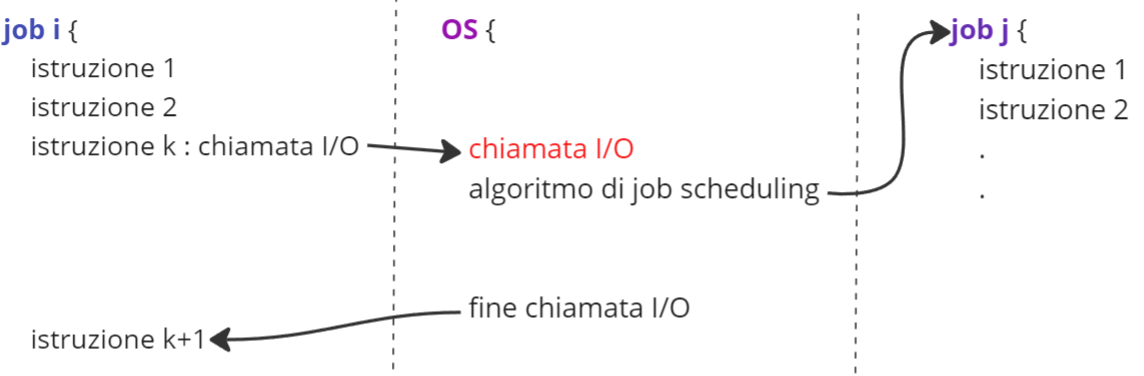
\includegraphics[width=0.7\textwidth ]{images/jobScheduling.png}
    }
\end{figure}
\\Assicurando un buon bilanciamento fra processi in esecuzione e chiamate I/O, tramite il job scheduling
la CPU non si arresterà mai ed avrà sempre un processo in esecuzione. Sorge però un altro problema, nel caso 
dovessimo avere un processo considerevolmente lungo, esso verrà eseguito per un \textit{tempo indeterminato} lasciando 
la CPU sempre occupata, si utilizza quindi un sistema di \textbf{time sharing}, in cui ad ogni processo 
è riservato un \textbf{tempo limitato}, in modo tale che esso se troppo lungo, viene momentaneamente arrestato per 
lasciare spazio ad altri processi (il tempo limite per ogni processo è stabilito dal sistema), essendo tali tempi 
molto bassi per la nostra percezione, tramite il time sharing l'utente avrà un'illusione di \textit{parallelismo} 
(solo apparente dato che una CPU può eseguire un solo processo alla volta).\\
È importante considerare che sospendere un processo per mandarne in esecuzione un altro 
(\textbf{context switch}) ha un suo costo, in quanto bisogna salvare lo \textit{stato} del processo precedente
salvando i valori contenuti nei registri e l'ultima istruzione da eseguire in modo da poterlo poi 
\textit{ripristinare} correttamente, per cui il tempo limitato dal sistema secondo il time sharing non deve 
essere troppo piccolo altrimenti si rischia di fare context switch troppe volte rispetto agli effettivi 
calcoli da eseguire.
\section{Architettura Necessaria per i Servizi dell'OS}\subsection{User e Kernel Mode}\label{user kernel}
Per mantenere un certo livello di sicurezza, all'interno dell'OS è possibile eseguire istruzioni in due 
modalità differenti, \textbf{user mode} e \textbf{kernel mode}. Alcune istruzioni sono più
\textit{sensibili}, se spostare il contenuto da un registro ad un altro (MOV) può essere fatto senza 
problemi, alcune istruzioni di interruzione dovrebbero richiedere un accesso privilegiato, per questo 
si vuole implementare la \textit{kernel mode}, che ha la possibilità di eseguire qualsiasi istruzione.
Fisicamente, si implementa un \textit{bit} che descrive appunto, tramite i suoi 2 stati, se si sta 
operando da utente, o in modalità kernel. Il sistema, in user mode, non può interagire direttamente 
con l'I/O, e non può manipolare il contenuto della memoria. Se l'utente necessita di eseguire operazioni 
in cui è necessaria la kernel mode, utilizza le \textbf{system call}, delle chiamate, che permettono 
la momentanea transazione in kernel mode per soddisfare la richiesta, per poi ritornare alla modalità 
utente.
\begin{wrapfigure}{l}{0.25\textwidth}
    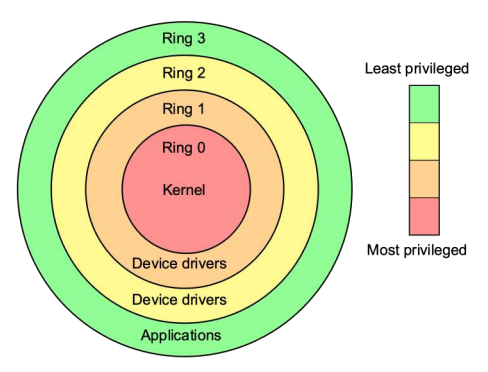
\includegraphics[width=1\linewidth]{images/protectionRings.png} 
    \caption{Protection Rings}
    \label{fig:wrapfig}
    \end{wrapfigure}
     \hphantom{,}\\ \hphantom{,}\\ \hphantom{,}\\Al minimo è necessario un \textit{bit} per i 2 stati, ma è possibile implementarne molteplici 
se si vogliono definire dei \textbf{protection rings}, ossia più stati di privilegi definiti a strati 
dove al livello 0 c'è il kernel, e gradualmente si hanno meno privilegi più il livello è alto. \hphantom{,}\\
\hphantom{,}\\ \hphantom{,}\\ \hphantom{,}\\ \hphantom{,}\\ \hphantom{,}\\
È anche necessario proteggere la memoria, limitanto ogni processo senza dargli la possibilità di poter
operare su tutta la memoria disponibile, a livello hardware si implementano due ulteriori registri, denominati
\textbf{base} e \textbf{limit}, quando un processo è in corso, ad esso verrà riservata una limitata partizione 
di memoria, in \textit{base} sarà contenuto l'indirizzo iniziale dalla quale parte la memoria disponibile, 
ed in \textit{limit} quello finale, in modo da fornire un \textit{range} di memoria utilizzabile. I valori di 
tali registri si aggiornano ad ogni \textit{context switch}, dato che ad ogni processo è assegnato il suo 
range [base,limit].
\subsection{Le System Call}
Come abbiamo già accennato, l'utente non può interagire direttamente con le istruzioni privilegiate, esistono 
appositamente le \textbf{system call} (o chiamate di sistema), esse richiedono al sistema operativo di eseguire 
determinate operazioni (come scrivere dati su un disco o inviare dati ad un interfaccia di rete), quindi esiste una 
lista di operazioni che l'utente può effettuare tramite esse, sono praticamente l'interfaccia tra l'utente ed il 
sistema operativo. Tali richieste sono definite \textbf{trap}, ossia eventi che causano lo switch da 
user a kernel mode, tali \textit{trap} non sono esclusivamente le system call, ma anche le 
\textbf{eccezioni} (errori generati dal software, privilegi assenti per un istruzione o tentata 
divisione per 0), e le \textbf{interruzioni} (errori generati dall'hardware, come la scadenza del tempo 
prefissato per un job tramite il timer).
\begin{figure}[h]
    \centering{
    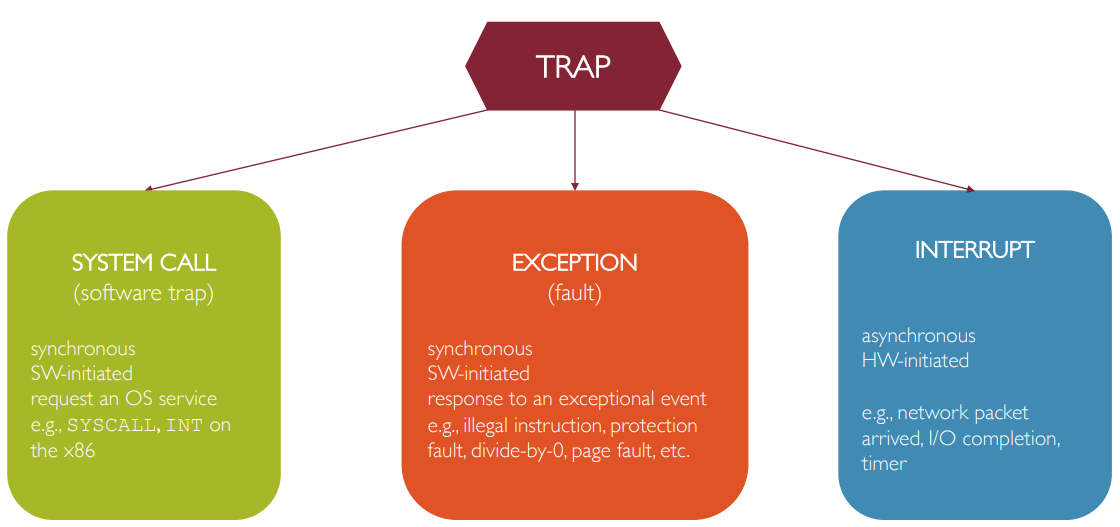
\includegraphics[width=0.7\textwidth ]{images/trapTerminologia.png}
    }
\end{figure}
\\Ci sono 6 categorie principali di system call :
\begin{itemize}
    \item \textbf{Controllo dei processi}
    \item \textbf{Gestione dei file}
    \item \textbf{Controllo dei dispositivi}
    \item \textbf{Manutenzione delle informazioni} 
    \item \textbf{Comunicazione tra processi} - per far comunicare due processi, o si utilizza un canale unico di 
    comunicazione tra i due (\textit{message passing}), oppure si fornisce un area di memoria condivisa tra due processi,
    che andrà poi liberata una volta finita la comunicazione(\textit{shared memory}).
    \item \textbf{Protezione} - forniscono agli utenti accesso temporaneo e limitato ai permessi.
\end{itemize}
\subsection{API per le System Call}
Usando le \textbf{API} (Application Programming Interface) al posto delle system call direttamente, è possibile 
fornire maggiore portatilità, e rendere un programma che necessita delle chiamate di sistema indipendente 
dall'hardware. Un API fornisce una libreria per un linguaggio di programmazione di alto livello (come il \textit{C}), 
che ci permette di chiamare funzioni che eseguiranno delle chiamate di sistema.
\begin{figure}[h]
    \centering{
    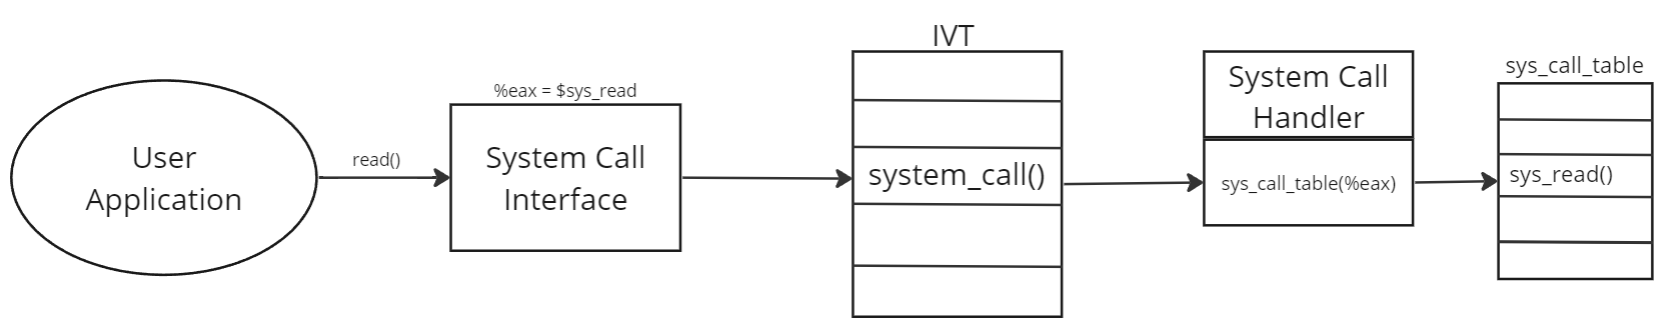
\includegraphics[width=0.9\textwidth ]{images/syscallFlow.png}
    }
\end{figure}
\newpage
Quando un utente chiama una funzione che richiede una syscall, viene generata un'interruzione, poi in un registro apposito 
(nell'immagine sovrastante "\textit{\%eax}") viene salvato il codice di quella specifica chiamata,
il segnale viene poi mandato alla \textbf{IVT} (Interrupt Vector Table), ossia un vettore all'interno 
del kernel che assegna ad ogni interruzione una causa. Quindi l'IVT, capisce che si tratta di una system call 
e manda il segnale al \textit{System Call Handler}, che si occupa di leggere il contenuto del registro 
prima citato ("\textit{\%eax}"), ed in base al codice, richiamare dalla \textit{System Call Table} la chiamata 
corretta.\\\hphantom{.}\\
Spesso, i parametri da passare non si limitano al codice identificativo della system call. Esistono 3 
diversi modi di passare parametri al sistema operativo :
\begin{itemize}
    \item Salvare parametri in dei \textbf{registri} (ma potrebbero esistere più parametri che registri).
    \item Salvare i parametri in \textbf{blocchi} o "tavole" in un'area di memoria dedicata, passando come 
    parametro nei registri l'indirizzo di tali blocchi.
    \item Passare i parametri inserendoli (\textit{push}) in uno \textbf{stack} dal programma, per poi farli 
    riprendere dallo stack (\textit{pop}) direttamente dal sistema operativo.
\end{itemize}
Il metodo migliore risulta quello dei \textit{blocchi} o dello \textit{stack}, dato che non hanno limiti sulla 
quantità di parametri che si possono possibilmente passare.\\\hphantom{.}\\
Le chiamate di I/O eseguite dalle system call possono essere \textbf{bloccanti} o \textbf{non bloccanti},
le chiamate bloccanti, interrompono il flusso del processo, lasciandolo in "stallo" finchè non si
riceveranno i dati richiesti dalla chiamata. Le chiamate non bloccanti invece, richiedono dati tramite 
le chiamate senza però interrompere il processo, sono quindi più difficili da implementare in quanto 
il programmatore deve considerare che dopo la chiamata, i dati richiesti potrebbero non essere 
da subito disponibili.\\\hphantom{.}\\
Come si è accennato precedentemente, risulta utile a livello fisico implementare un \textbf{timer} che 
segna semplicemente l'orario del giorno corrente (detto \textit{time stamp}), esso è utile allo 
\textit{scheduler}\ref{scheduling}, ad esempio, può generare un interruzione ogni 100 \textit{microsecondi}, in modo che 
lo scheduler possa prendere il sopravvento sul processo per poi decidere quale altro job va eseguito.\\\hphantom{.}\\
Alcune istruzioni sono dette \textbf{atomiche}, ossia, non possono essere fermate dalle interruzioni, le architetture 
che implementano tali istruzioni devono far si che esse vengano eseguite per intero, piuttosto, vengono
totalmente abortite. Per eseguirle è possibile definirle nel linguaggio macchina come istruzioni speciali 
che sono nativamente eseguite in maniera atomica, oppure, è possibile \textit{disabilitare} momentaneamente 
tutte le interruzioni.
\subsection{La Memoria Virtuale}
La \textbf{memoria virtuale} è un \textit{astrazione} della memoria fisica, da l'illusione ad un processo di 
avere illimitato spazio di memoria per lavorare, e consente ad esso di non essere totalmente caricato 
in memoria, caricandolo appunto nella memoria virtuale. Tale memoria è implementata sia a livello 
hardware(MMU) che software(OS) :
\begin{itemize}
    \item \textbf{MMU} - è il componente che si occupa di tradurre gli indirizzi virtuali in indirizzi fisici.
    \item \textbf{OS} - è responsabile di gestire lo spazio degli indirizzi virtuali.
\end{itemize}
Un sistema a 64 \textit{bit}, è capace di indirzzare \(2^{64}\) entry, gli indirizzi virtuali sono 
suddivisi in blocchi della stessa dimensione, chiamati \textbf{pagine}, le pagine che non vengono caricate 
nella memoria principale, vengono salvate sul disco. Facendo ciò si fornisce ad un processo una quantità \(n\) di 
indirizzi virtuali, che sono salvati sia in memoria che su disco, essi vengono mappati tramite quella che si chiama 
\textbf{page table}, e si utilizza anche una cache chiamata \textbf{TLB} (Translation Look-aside Buffer), che salva 
i recenti "indirizzamenti" per potervi accedere più rapidamente. L'OS deve considerare quali pagine sono 
salvate sul disco, e quali sulla memoria principale.
\subsection{Design di Noti Modelli di Sistema Operativo}
La struttura interna di un sistema operativo può variare largamente in base alle necessità di utilizzo 
di tale sistema, è necessario separare quelle che sono le \textbf{politiche} del sistema 
(Le funzioni che deve svolgere) dal suo \textbf{meccanismo} (La possibile implementazione di tali funzioni).
Tale distinzione ci permette di rendere l'OS più flessibile alle modifiche, riusabile per implementare nuove 
politiche, e stabile. I primi sistemi operativi erano totalmente implementati in linguaggio macchina, ciò 
consentiva ad essi di essere molto efficenti, di contro però, erano limitati esclusivamente all'hardware sulla 
quale erano scritti. I sistemi operativi odierni hanno esclusivamente una piccola porzione scritta in 
linguaggio macchina, il corpo principale è scritto in \textit{C}, ed i programmi di sistema possono essere scritti 
in \textit{C++}, ed altri linguaggi di scripting come \textit{Python}. Un OS dovrebbe essere partizionato 
in sotto-sistemi, ognungo con compiti ben definiti. Esistono varie strutture di sistema operativo :
\begin{itemize}
    \item \textbf{Simple Structured} - Un sistema non modulare, nella quale non esiste distinzione tra 
    user e kernel. Risulta facile da implementare, ma pecca di rigidità e sicurezza. Un esempio di un OS che 
    adopera tale struttura è \textit{MS-DOS}.
    \item \textbf{Kernel Monolitico} - Un sistema strutturato in modo che sia tutto un grande ed unico processo, con
    tutti i servizi che vivono nello stesso spazio di indirizzamento. Risulta efficente,
    ma essendo un unico processo non ci sono limiti di visibilità tra diverse componenti, risulta 
    quindi poco sicuro. Un esempio di un OS che adopera tale struttura è \textit{UNIX}.
    \item \textbf{Layered Structured} - Un sistema diviso in \(n\) strati, dove il livello 0 rappresenta l'hardware, 
    ed ogni livello \(k\) implenta delle funzionalità che potranno essere riutilizzate dal livello \(k+1\) per 
    implementare nuovi programmi. Essendo modulare, risulta portatile, ma bisogna implementare dei canali di 
    comunicazione fra i vari strati.
    \item \textbf{Micro Kernel} - È l'opposto del \textit{Kernel Monolitico}. Nel kernel si inseriscono 
    esclusivamente le funzionalità di base, tutto il resto sarà gestito dalle applicazioni a livello utente. Risulta
    sicuro ed estendibile, ma pecca nella comunicazione. 
    \item \textbf{Loadable Kernel} - Ogni componente è separata, l'approccio risulta simile ai linguaggi 
    di programmazione \textit{object-oriented}. I moduli vengono caricati separatamente all'interno del 
    kernel. Ogni componente comunica con le altre tramite un interfaccia, è simile al \textit{Layered Structured},
    ma più flessibile.
\end{itemize}
È importante in base alla struttura utilizzata, provvedere al giusto hardware da implementare. I sistemi 
moderni utilizzano per lo più approcci ibridi.\newpage
\section{La Gestione dei Processi}
Definiamo la differenza tra \textbf{programma} e \textbf{processo} :
\begin{itemize}
    \item Programma - rappresenta l'eseguibile di un certo applicativo, contiene le istruzioni da eseguire ed 
     è contenuto sul disco fisso. 
     \item Processo - rappresenta l'istanza del programma che viene avviato e caricato sulla memoria principale,
     una volta avviato, l'OS si occuperà di tale processo. 
\end{itemize}
Quindi un programma viene \textit{istanziato} in un processo, che è un entità dinamica e viene eseguito 
dalla CPU, ogni processo è un entità indipendente, e possono coesistere due processi istanza dello stesso
programma. Ad ogni processo viene assegnata la sua quantità di memoria disponibile, e le sue istruzioni sono 
eseguite in maniere sequenziale. Il sistema operativo si occupa di creare, distruggere, e gestire gli stati 
dei processi, dedica ad essi la stessa quantità di memoria virtuale, ed il numero di indirizzi disponibili dipende 
dall'architettura della macchina (ad esempio, con un processore a 32 \text{bit}, si hanno \(2^{32}\) indirizzi disponibili).
\\\hphantom{.}\\
Quando si crea un processo, ad esso viene assegnata una quantità di memoria divisa in 4 unità logiche :
\begin{itemize}
    \item \code{Text} - contiene le istruzioni eseguibili, ossia il risultato della compilazione.
    \item \code{Data} - contiene le variabili globali o statiche non inizializzate, o inizializzate a 0.
    \item \code{Stack} - struttura LIFO utilizzata per memorizzare i dati ed i parametri necessari alle chiamate di funzioni.
    \item \code{Heap} - struttura dati utilizzata per l'allocazione dinamica della memoria.
\end{itemize}
Per ogni processo quindi, esiste tale area di memoria suddivisa in 4 unità. Lo \textbf{Stack} ha su di esso due 
operazioni, \code{push()} e \code{pop()}, ed un registro dedicato chiamato \textit{Stack Pointer} memorizza 
l'indirizzo alla cima dello stack. Ogni funzione utilizza una porzione dello stack che viene denominata 
\textbf{Stack Frame}, quindi quando si chiamano funzioni dentro altre funzioni, coesisteranno simultaneamente 
più stack frame, anche se esclusivamente uno di essi sarà attivo, ossia quello sulla quale risiede lo 
stack pointer (lo stack "cresce" verso il basso, quindi l'ultima funzione chiamata sarà quella attiva). 
\\\hphantom{.}\\ Lo stack frame contiene :\begin{itemize}
    \item Parametri della funzione ed indirizzo di ritorno
    \item Puntatore al precedente dello stack frame precedente
    \item Variabili locali
\end{itemize}
Quando si chiama una funzione che richiede dei parametri,
essi verrano inseriti (\code{push()}) nello stack, il valore dello stack pointer verrà aggiornato, e verrà inserito nello 
stack anche l'indirizzo dell'istruzione di ritorno. Il problema è che lo stack pointer viene aggiornato ogni 
volta che si chiama una nuova funzione, quindi si usa un altro puntatore detto \textit{Base Pointer} sul fondo 
dello stack, che rimane fisso per ogni stack frame senza aggiornarsi, differentemente dallo stack pointer che per 
forza di cosa, si aggiorna ogni qual volta viene aggiunto un nuovo valore.\newpage \subsection{Stati di un Processo}
Un processo in esecuzione può ritrovarsi in uno dei seguenti 5 \textbf{stati} : \begin{itemize}
    \item \code{new} - Il sistema operativo ha indirizzato le strutture per eseguirlo.
    \item \code{ready} - Il processo ha tutte le risorse necessarie per iniziare o ricominciare ad essere eseguito.
    \item \code{running} - Il processo è in esecuzione sulla CPU.
    \item \code{waiting} - Il processo è sospeso, in attesa che venga soddisfatta una chiamata/richiesta che necessita per poter continuare.
    \item \code{terminated} - Il processo è concluso, l'OS può liberare la memoria dalle risorse che utilizzava.
\end{itemize}
\begin{figure}[h]
    \centering{
    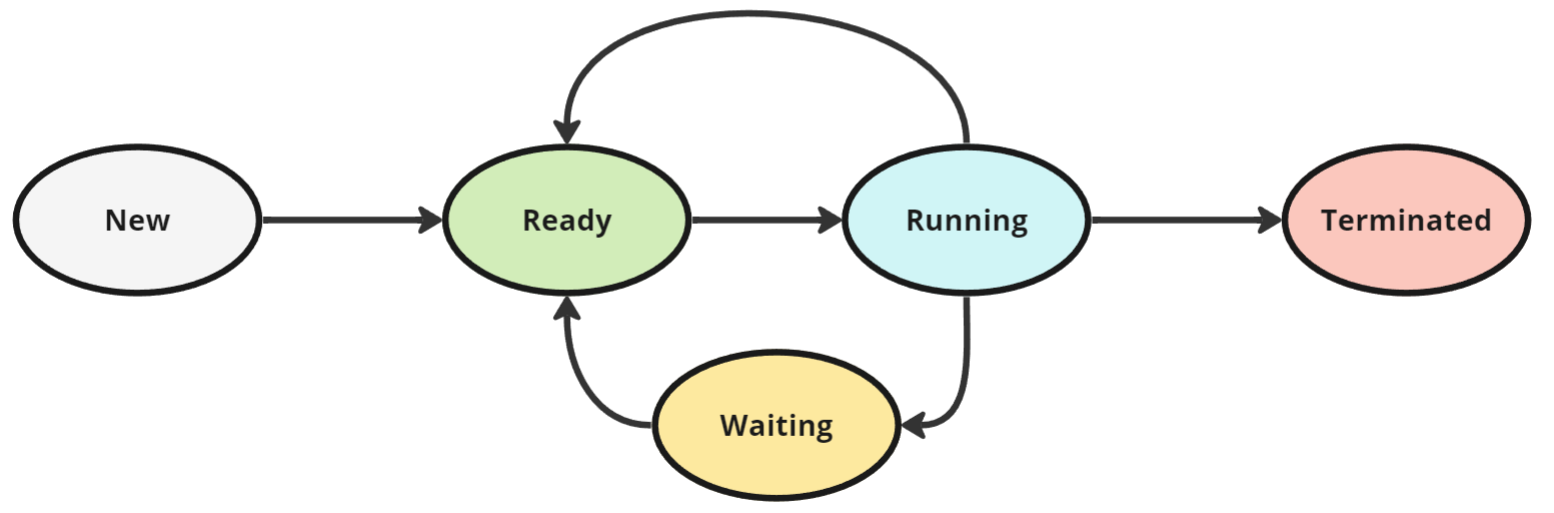
\includegraphics[width=0.7\textwidth ]{images/processStates.png}
    }
\end{figure}
\subsection{Creazione dei Processi}
Il sistema operativo per creare nuovi processi utilizza delle opportune chiamate di sistema. Per convenzione, 
un processo \textit{Parent} (detto anche padre) è quello dalla quale si esegue la chiamata per generare nuovi processi, detti 
\textit{Figli}. Ogni processo ha due valori interi utilizzati per identificare se stesso: \code{PID}, ed 
il suo parent : \code{PPID}. In sistemi come Unix, il process scheduler ha come PID=0, esso inizializza 
come prima cosa un processo noto come \code{init}, che ha PID=1, e si occuperà di creare tutti i processi, sarà 
quindi il parent primario. I processi vengono creati tramite una chiamata di sistema denominata \code{fork()}.
Ogni processo crea più figli, generando una struttura gerarchica ad albero.\\
\hphantom{}\\ La chiamata \code{fork()} nello 
specifico, non crea un nuovo processo, ma crea un processo \textit{clone}, identico a quello chiamante, si utilizza 
poi una chiamata \code{exec()}, che prendendo come parametri l'indirizzo in memoria di un determinato programma, 
sostituirà al processo corrente le istruzioni del programma nuovo che si vuole eseguire. Sarà quindi la congiunzione 
di tali chiamate \code{fork()} ed \code{exec()} a generare un nuovo processo.
\\\hphantom{}\\ 
Quando un processo padre genera un figlio, ha due possibili opzioni :\begin{itemize}
    \item Arrestare la sua esecuzione, ed attendere che il processo figlio appena generato termini prima di ricominciare,
    tramite la chiamata \code{wait()}.
    \item Continuare la sua esecuzione, in maniera concorrente con il suo processo figlio.
\end{itemize}
Vediamo come un programma si occupa di generare un nuovo processo tramite la chiamata di sistema :\newpage
\begin{lstlisting}[language=C]
    #include <sys/types.h>
    #include <stdio.h>
    #include <unistd.h>
    
    int main(){
        pid_t pid;
        /* fork a child process */
        pid = fork();

        if(pid<0){
            /* error occurred */
            fprint("Fork Failed");
            exit(-1);
        }

        else if(pid==0){
            /* child process */
            execlp("bin/ls","ls",NULL);
        }

        else{
            /* parent process */
            wait(NULL);
            printf("Child Complete");
            exit(0);
        }
    }
\end{lstlisting}
Si osservi il codice sopra mostrato. Quando viene eseguito un \code{fork()} e creato un clone, i due processi 
padre e figlio differiranno esclusivamente per il loro PID. La funzione \code{fork()} ritorna il PID del 
processo appena clonato(quindi il padre avrà salvato nella variabile, il PID del figlio)
, il processo figlio, avrà la variabile pid=0, per questo si entrà nel blocco 
di codice che si occuperà di fare l'\code{exec()} sostituendo le istruzioni con quelle del 
programma presente all'indirizzo \code{"bin/ls"}, generando così un nuovo processo. Se il PID è diverso da 0, 
il programma eseguirà una \code{wait()}, aspettando che il processo figlio termini, prima di ricominciare.
\begin{figure}[h]
    \centering{
    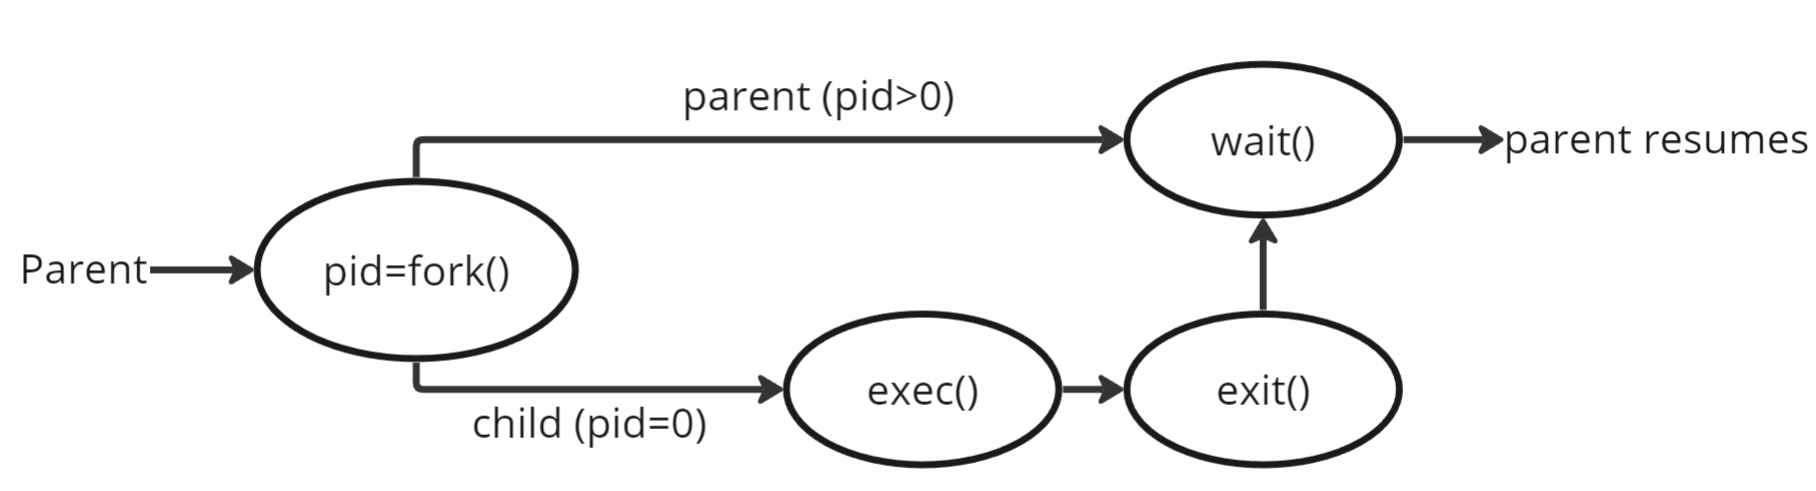
\includegraphics[width=0.9\textwidth ]{images/forkGraph.png}
    }
\end{figure}
Sarà quindi il programma scritto dall'utente a dover implementare la logica adeguata (tramite la 
lettura dei PID) per capire se il processo attualmente in esecuzione è quello padre o quello figlio.
\\\hphantom{}\\ 
Un processo può esplicitamente richiedere la sua terminazione tramite la chiamata di 
sistema \code{exit()}, dando un codice di uscita, che per convenzione è 0 quando tale processo 
ha terminato la sua esecuzione senza errori, altrimenti -1, oppure può essere terminato in maniere 
forzata dal suo processo padre. Un processo non può esistere senza padre,
se un processo padre termina ma vi sono ancora dei processi figli in esecuzione, essi, detti 
processi \textit{orfani}, vengono ereditati dal processo \code{init}, che si occuperà di terminarli.
Quando un processo termina, lo spazio dedicato alle sue risorse viene liberato.
\subsection{Scheduling dei Processi}
Un sistema operativo deve far conto a due obbiettivi : \begin{itemize}
    \item far si che la CPU stia costantemente eseguendo processi 
    \item avere un tempo di risposta accettabile per i programmi che interagiscono con l'utente
\end{itemize}
Lo scheduler si occupa di decidere quale processo eseguire venendo in contro a tali obbiettivi, anche se 
essi possono entrare in conflitto fra loro. Il sistema operativo salva tutti i PCBs\footnote{
 Process Control Block
} dei processi in delle code, ci sono 5 code, una per ogni possibile stato. Quando un processo cambia stato, 
il suo PCB viene eliminato dalla coda precedente ed inserito nella nuova coda corrispondente. Ovviamente, 
nella \textit{Running Queue} vi può essere un solo processo per volta (in sistemi con architetture single core).
Nelle altre code, non ci sono limiti teorici di dimensioni.
\\\hphantom{}\\ 
Esistono due tipi di scheduler.\begin{itemize}
    \item Il \textbf{long-term scheduler} si occupa di selezionare i processi da eseguire dalla memoria secondaria 
    (ad esempio, il disco) e di caricarli in memoria principale, viene eseguito poco frequentemente.
    \item Lo \textbf{short-term scheduler} invece, si occupa di selezionare i
     processi dalla coda dei pronti e di assegnarli alla CPU per l'esecuzione, viene eseguito molto frequentemente,
     circa ogni 50-100 millisecondi.
\end{itemize}
Abbiamo già definito l'operazione di \textit{Context Switch}, ossia quella di interrompere un processo per 
eseguirne un altro. Tale operazione risulta costosa in termini computazionali, dato che è necessario salvare 
lo stato del processo da interrompere e caricare lo stato del processo da eseguire dai loro rispettivi 
PCB. Il context switch è quindi operazione da eseguire solo quando necessario, quando avviene un interruzione, oppure 
quando un processo impiega troppo tempo generando un interruzione del timer. I processi che utilizzano principalmente 
la CPU per eseguire esclusivamente calcoli (talvolta pesanti), che quindi richiedono più tempo per essere 
completati, senza però fare richieste di I/O, sono detti \textit{CPU-bound processes}.
\\\hphantom{}\\ 
Il tempo che impiega la CPU per fare context switch è "sprecato" dato che non si stanno effettuando 
calcoli utili all'esecuzione dei processi, quindi a seconda delle disponibilità, è possibile implementare 
un quanto di tempo massimo dedicato ad ogni processo, a seconda delle esigenze:\begin{itemize}
    \item Un quanto di tempo minore farà si che si eseguiranno più context switch, aumentando la responsività.
    \item Un quanto di tempo maggiore risulterà in meno context switch, minimizzando il tempo perso della CPU, massimizzandone
    il suo utilizzo.
\end{itemize}
\subsection{Comunicazione fra processi}
Due processi possono essere fra loro :  \begin{itemize}
    \item \textbf{cooperativi} - possono influire o venire influiti da altri processi per operare su computazioni comuni.
    \item \textbf{indipendenti} - operano in maniera concorrente sul sistema e non si influenzano fra loro.
\end{itemize}
Un processo particolarmente complesso può essere scomposto in più processi \textit{cooperativi}, 
è necessario predispore i processi cooperativi di adeguati canali di comunicazione, ci sono due possibili 
modi di farli comunicare :\begin{itemize}
    \item \textbf{Message Passing} - è il metodo più lento, dato che per ogni trasferimento, avviene tramite
    una system call, ma è semplice da mettere in atto quindi preferibile se la quantità o la frequenza dei messaggi 
    non è particolarmente elevata.
    \item \textbf{Shared Memory} - è più complesso da mettere in atto e non funziona perfettamente quando si lavora 
    su più computer, non richiede però l'utilizzo delle system call ed è quindi preferibile quando si devono 
    trasferire grandi quantità di informazioni sullo stesso computer.
\end{itemize}
Nel sistema \textit{Shared Memory} viene creato uno spazio di memoria condiviso per due processi differenti, inizialmente 
tale memoria appartiene al PCB di un solo processo, tramite una system call viene poi resa pubblica e disponibile 
ad altri processi, che possono fare delle system call per accedere ad essa.
\\\hphantom{}\\ 
Nel \textit{Message Passing}, il sistema operativo deve implementare delle specifiche system call adibite 
all'invio e ricezione dei messaggi, un collegamento va stabilito tra due processi cooperanti. Il processo 
mittente deve poter identificare il processo destinatario, è possibile creare un canale "uno ad uno" per 
ogni coppia di processi comunicanti, oppure creare delle "porte" condivise dove più processi possono 
comunicare, e trasferire informazioni su tali porte che potranno essere lette da ogni processo. Tali messaggi 
ovviamente occupano spazio in memoria,
solitamente vanno in una coda, 
ci sono 3 diversi modi di gestire la coda ad essi riservata :
\begin{itemize}
    \item \textbf{Zero Capacity} - I messaggi non hanno una coda nella quale vengono salvati, quindi il mittente 
    si blocca e non può inviare altri messaggi finche il destinatario non risponde.
    \item \textbf{Bounded Capacity} - I messaggi vengono salvati in una coda con una
     capacità di memoria finita predeterminata, quindi i mittenti potranno inviare messaggi affinché la coda 
     non sarà piena.
     \item \textbf{Unbounded Capacity} - La coda ha una capacità (teoricamente) infinita, quindi i mittenti 
     potranno inviare messaggi senza blocchi.
\end{itemize} 
\begin{figure}[h]
    \centering{
    \includegraphics[width=0.65\textwidth ]{images/processCommunication.eps}
    }
\end{figure}
\subsection{Algoritmi di Scheduling}
Vediamo in questo paragrafo quali sono alcuni dei criteri presi in considerazione dagli scheduler per selezionare 
il prossimo processo dalla coda pronti che andrà in esecuzione. Lo scheduler deve far si che si alternino in continuazione 
processi CPU-bound e processi che fanno operazioni di I/O, tenendo in considerazione che gli accessi alla memoria 
richiedono svariati cicli di clock, togliendo tempo al calcolo effettivo.\\
\hphantom{text}\\Ci sono 4 possibili situazioni in cui interviene lo short term scheduler per prendere un processo 
dalla coda pronti :\begin{enumerate}
    \item  Quando un processo passa dallo stato running allo stato waiting (ad esempio quando vi è una system call).
    \item  Quando un processo passa dallo stato running allo stato ready
     (quando scade il timer che determina il tempo massimo assegnato ad ogni processo).
     \item  Quando il processo passa dallo stato waiting allo stato ready
      ( il processo interrotto perché ha richiesto una risorsa, vede tale risorsa diventare disponibile).
      \item  Quando viene creato un nuovo processo ed entra nella coda dei processi pronti, oppure quando un processo termina.
\end{enumerate}
Si noti come, nei casi 1 e 4, lo scheduler è costretto ad intervenire, in quanto la CPU necessita di un nuovo 
processo da eseguire, nei casi 2 e 3 invece, l'intervento non è necessario, ed è a discrezione dello scheduler 
se intervenire o meno.\\Gli scheduler che intervengono esclusivamente quando è necessario, si dicono 
\textbf{Non-preemptive}, quelli che invece, intervongono anche nei casi 2 e 3, sono detti \textbf{Preemptive}.\\ 
\hphantom{text}\\Uno scheduler \textit{Preemptive} può essere problematico se agisce in situazioni delicate (Ad esempio, 
mentre il Kernel sta eseguendo una system call), per questo prima di eseguire un interruzione, l'OS si occupa di 
accertarsi che una chiamata di sistema sia completata prima di eseguire il blocco (se necessario, si interrompono 
momentaneamente le interruzioni).\\\hphantom{text}\\
È importante sapere che il modulo dello scheduler che si occupa specificamente di far eseguire 
alla CPU il processo selezionato è noto con il nome di \textbf{Dispatcher}, si occupa di fare context switch,
passare alla user mode, e "saltare" all'indirizzo di memoria dell'ultimo programma caricato.
\subsubsection{Criteri e Politiche dello Scheduling}
Introduciamo adesso alcune notazioni e definizioni importanti riguardo il calcolo dei tempi che un processo 
impiega sulla CPU.\begin{itemize}
    \item \textbf{Arrival Time} (\(T_{arrival}\)) : L'istante in cui un processo arriva nella coda pronti.
    \item \textbf{Completion Time}  (\(T_{completion}\)) : L'istante in cui un processo completa la sua esecuzione.
    \item \textbf{Burst Time:}  (\(T_{burst}\)) : Il tempo totale nella quale il processo è in esecuzione sulla CPU.
    \item \textbf{ Turnaround Time} (\(T_{turnaround}\))  : La differenza fra il Completion Time e l'Arrival Time, definita 
    come \(T_{completion}-T_{arrival}\) .
    \item \textbf{ Waiting Time} (\(T_{waiting}\)) : La differenza fra il Turnaround Time ed il Burst Time, definita 
    come \(T_{turnaround}-T_{burst}\) .
\end{itemize}
Ci sono diversi criteri da poter prendere in considerazione quando si scrive una algoritmo di scheduling, ed in 
base a tali criteri, esistono algoritmi migliori di altri, tali criteri sono :\begin{itemize}
    \item \textbf{Utilizzo della CPU} - Il tempo in cui la CPU è occupata ad eseguire calcoli, idealmente, dovrebbe 
    essere occupata il 100\(\%\) del tempo, l'obbiettivo è quindi di \textit{massimizzare} tale utilizzo.
    \item \textbf{Throughput} - Il numero di processi da completare per unità di tempo, l'obbiettivo è quindi di \textit{massimizzare} tale numero.
    \item \textbf{Tournaround time} - L'obbiettivo è quello di \textit{minimizzare} il tempo impiegato da un processo, 
    dalla sua selezione da parte dello scheduling fino al completamento (includendo lo Waiting Time).
    \item \textbf{Waiting time} - L'obbiettivo è quello di \textit{minimizzare} il tempo che un processo 
    rimane fermo nella coda, in attesa di essere selezionato dallo scheduler.
    \item \textbf{Response time} - Il tempo che interocorre fra la richiesta di un comando, e la risposta ad esso, l'obbiettivo 
    è quello di \textit{minimizzare} tale tempo per rendere il sistema più interattivo e responsivo.
\end{itemize}
Idealmente sarebbe ottimo scegliere un algoritmo di scheduling che soddisfa 
tutte le richieste appena elencate, ovviamente in una situazione reale, la 
massimizzazione di certi criteri porta svantaggio agli altri, rientra 
quindi il concetto di \textit{trade-off}, sceglieremo quindi un certo 
algoritmo di scheduling in grado di soddisfare solo un certo tipo di 
politiche.\begin{itemize}
    \item Minimizzare il response time medio fa si che l'utente 
    riceva l'output il più rapidamente possibile, minimizzare il tempo massimo 
    di response time invece, previene dagli scenari in cui un processo 
    ha un response time molto più alto rispetto agli altri, minimizzare 
    la varianza invece, rende il response time dei processi più "predicibile" 
    dall'utente, queste politiche son tipiche dei \textbf{sistemi interattivi}.
    \item Massimizzare il throughput si traduce in un utilizzo più efficente 
    delle risorse di sistema, e minimizzare il waiting time da ad ogni processo 
    la stessa quantità di tempo da spendere sulla CPU (di contro, potrebbe 
    aumentare la media del response time), queste politiche son tipiche 
    dei \text{sistemi batch}\footnote{
        tipo di sistema in cui i processi vengono eseguiti  in gruppi o lotti. Invece di eseguire ogni processo in modo interattivo e immediato, un batch system raccoglie una serie di processi o comandi e li esegue in sequenza, senza richiedere l’interazione dell’utente durante l’esecuzione.
    }.
\end{itemize}
Vediamo adesso il funzionamento generale di alcuni algoritmi di scheduling noti,
i quali possono essere preemptive oppure non-preemptive.
\subsubsection{First Come First Served (FCFS)}
Tale algoritmo funziona, ed è implementato come una coda 
\textit{First-In-First-Out}, è quindi molto semplice, in quanto manda 
in esecuzione i processi in ordine di arrivo, lo scheduler entra in funzione 
solamente quando un processo in esecuzione fa una richiesta 
di I/O (oppure termina la sua esecuzione).\acc I processi non sono limitati 
da un tempo massimo quindi possono rimanere in esecuzione sulla CPU 
per un tempo indeterminato, è quindi uno scheduler \textit{non-preemptive}. 
\begin{itemize}
    \item \textbf{Pro} - Risulta molto semplice da implementare.
    \item \textbf{Contro} - Il tempo di attesa (waiting time) è molto 
    variabile. Vi è poca alternanza di processi I/O-bound e processi 
    CPU-bound dato che un processo che fa richiesta di I/O potrebbe trovarsi 
    dopo (e quindi attendere la terminazione) di un processo che 
    impiegherà molto tempo sulla CPU.
\end{itemize}
\subsubsection{Round-Robin (RR)}
È un algoritmo simile al FCFS, solo che impone un limite di tempo 
(detto quanto temporale) ai processi che impiegano troppo tempo 
sulla CPU. Quando un job viene assegnato alla CPU, parte un timer 
(implementato a livello hardware). \acc Se il processo termina prima della scadenza 
del timer, lo scheduler manda in esecuzione il prossimo come un semplice 
FCFS, se invece il timer scade durante l'esecuzione del processo, 
lo scheduler interviene dando in esecuzione alla CPU il prossimo processo, quello 
interrotto invece verrà re-inserito in fondo alla coda, è quindi un sistema 
\textit{preemptive}.\acc Come implicato, i processi pronti sono gestiti 
in una coda circolare, è uno scheduler equo in quanto garantisce a tutti 
i processi lo stesso tempo di esecuzione sulla CPU. Le performance di questo 
algoritmo sono sensibili alla durata del quanto temporale scelto, se il tempo 
del quanto è molto grande, l'algoritmo si comporterà come un FCFS, 
se troppo piccolo, verranno fatti troppi context switch.
\subsubsection{Shortest-Job-First (SJB)}
L'idea, è di dare la priorità ai processi che hanno il 
"carico di lavoro stimato" più piccolo sulla CPU, con carico di lavoro, si 
intende il tempo che impiegheranno in esecuzione (burst time), prima della prossima 
richiesta di I/O o della terminazione stessa.\begin{itemize}
    \item \textbf{Pro} - È ottimale quando l'obbiettivo è quello di 
    minimizzare il tempo di attesa.
    \item \textbf{Contro} - È quasi impossibile sapere con precisione 
    quale sia il prossimo processo con il minor carico di lavoro da eseguire.
    Inoltre, vi è il rischio che i processi con un carico di lavoro 
    elevato entrino nella condizione di \textit{starvation}\footnote{
        Restano nella coda senza mai essere selezionati dallo scheduler, 
        in quanto hanno bassa proprità di essere selezionati.
    }.
\end{itemize}
Come si può però "predirre" il tempo che un processo impiegherà sulla 
CPU? L'idea, è quella di basarsi sui tempi di esecuzione dei processi 
precedenti, tramite una tecnica nota come \textbf{exponential smoothing}.\begin{center}
    \(x_t=\) Tempo attuale sulla CPU del \(t\)-esimo processo (valore noto). 
    \\\(s_t=\)  Tempo stimato sulla CPU del \(t\)-esimo processo (valore noto).
    \\Dati \(x_t\) e \(s_t\), vogliamo stimare il tempo di attesa del prossimo processo, 
    ossia \(s_{t+1}\). \\
    Sia \(\alpha\) un coefficente reale : \(\alpha\in [0,1]\), la predizione sarà :\\
\(s_{t+1}=\alpha\cdot x_t+(1-\alpha)\cdot s_t\)
\end{center}
Facciamo alcune osservazioni :\acc
    \(\alpha=0\implies s_{t+1}=s_t\implies\) Si ignora il tempo misurato del processo 
    precedente. e si assume un tempo di lavoro costante per tutti i processi.\acc 
    \(\alpha=1\implies s_{t+1}=x_t\implies\) Si assume che il tempo di lavoro 
    del prossimo processo sia lo stesso del processo precedente.\acc 
Solitamente, si decide che \(\alpha=\dfrac{1}{2}\). Tale algoritmo può essere implementato 
sia in maniera \textit{preemptive} che \textit{non-preemptive} : \begin{itemize}
    \item Una volta che un processo viene assegnato, rimane sulla CPU fino alla prossima 
    interruzione (o terminazione).
    \item Quando un nuovo processo arriva nella coda pronti, si controlla se 
    esso ha un tempo di lavoro stimato maggiore del processo in esecuzione, se si, 
    viene eseguito lo switch.
\end{itemize}
\subsubsection{Priority Scheduling} 
È il caso generale del SJF, in cui ad ogni job viene assegnato un 
grado di priorità in base a certi parametri, e lo scheduler 
prediligerà i processi con la priorità più alta (nel caso del SJF, 
più il carico di lavoro è basso, più il processo è prioritario). Il livello 
di priorità non è altro che un valore intero, mantenuto in un 
certo range (usualmente, più il numero è basso più la priorità 
è alta).\acc Le politiche possono essere assegnate :\begin{itemize}
    \item \textbf{Internamente} - Il grado di priorità è assegnato 
    dal sistema operativo considerando politiche e criteri interni come il tempo di lavoro 
    sulla CPU, l'alternanza fra richieste di I/O ed esecuzione ecc..
    \item \textbf{Esternamente} - Il grado di priorità è assegnato dall'utente 
    basandosi su criteri totalmente arbitrari in base all'importanza 
    del processo.
\end{itemize}
Come visto prima, tale algoritmo può essere implementato 
sia in maniera \textit{preemptive} che \textit{non-preemptive}.\acc
Si è accennato precedentemente della \textbf{starvation}, ossia della condizione 
in cui un processo con bassa priorità, rischia di non essere mai selezionato in 
quanto surclassato da processi sempre con gradi di priorità superiori. La 
soluzione più ovvia risulta essere quella denominata con \textbf{aging}, ossia, 
l'operazione di aumentare il grado di priorità di un processo nel tempo, in modo che,
anche i processi poco prioritari, con l'andare avanti nel tempo verranno prima o poi 
schedulati.
\subsubsection{Multi-Level-Queue (MLQ)}
L'insieme dei processi viene diviso in partizioni, in base alla categoria 
di ogni processo (ad esempio, una categoria per i processi grafici, una per i processi 
 correlati all'audio, ecc..), e si applicano algoritmi diversi di scheduling 
 su ogni categoria. \acc Un esempio è l'applicazione della \textbf{Strict Priority}, 
 in cui i processi vengono divisi in diverse code in base ad un grado di priorità 
 deciso, e poi ogni singola coda avrà il proprio algoritmo di scheduling, ad esempio, 
 il RR, dove ogni coda ha un quanto temporale diverso dalle altre.
  \acc \textbf{Attenzione} : Nessun processo può passare da una coda ad un altra.
  \begin{figure}[h]
    \centering{
    \includegraphics[width=0.8\textwidth ]{images/expSmoothing.eps}
    }
\end{figure}\\
\subsubsection{Multi-Level-Feedback-Queue (MLFQ)}
L'idea è simile alla normale MLQ, solo che in questo caso, i processi possono \textit{muoversi fra 
le diverse code}. Ciò può essere necessario in diverse situazioni, per rendere lo scheduling più 
adattivo, ad esempio : \begin{itemize}
    \item Un processo cambia le sue caratteristiche, alternandosi nell'essere un CPU-Bound ed un processo che 
    fa molte richieste di I/O.
    \item Un processo può rimanere in attesa troppo tempo, quindi l'aging interviene spostandolo in una coda con 
    priorità maggiore.
\end{itemize}
Di default, i processi vengono tutti inizializzati nella coda con priorità più alta, che ha a sua volta il 
quanto temporale più corto. Se il tempo a disposizione scade, vengono spostati nella coda successiva, di un grado 
di priorità inferiore, e così via. \acc Se il quanto temporale di un processo invece non lo blocca (ad esempio, il processo 
si interrompe con richieste di I/O sempre prima che il suo tempo a disposizione scada), allora viene spostato 
nella coda superiore, con priorità più alta. I processi che richiedono molto calcolo e tempo sulla CPU, cadranno rapidamente 
nelle code più "basse" con meno priorità, differentemente, i processi che fanno molte richieste di I/O 
rimarranno nelle code più "alte".\acc 
Uno scheduling MLFQ è estremamente flessibile, ma anche molto complesso da implementare, bisogna gestire svariati 
parametri, quali : \begin{enumerate}
    \item Il numero delle code.
    \item L'algoritmo di scheduling per ogni coda. 
    \item Le politiche adoperate per spostare i processi fra le code. 
    \item Il metodo utilizzato per determinare in quale coda un processo dovrebbe essere inizializzato.
\end{enumerate}
Questo algoritmo, si comporta in maniera simile al SJF in termini di tempo di attesa, in quanto cerca di privilegiare i 
processi corti, potrebbe quindi essere poco equo.
\subsubsection{Lottery Scheduling} 
Esiste un tipo di scheduling inusuale basato sulla casualità. Ad ogni processo, viene assegnato un certo 
numero di "ticket". Ad ogni intervallo di tempo, si estrae \textbf{casualmente} (con probabilità uniforme) un 
numero. Il processo in possesso del ticket con il numero estratto, verrà schedulato. Con l'andare avanti del tempo, 
per la \textit{legge dei grandi numeri}, prima o poi ogni processo verrà schedulato. \acc 
Risulta opportuno dare più ticket ai processi più corti, in modo che possano essere schedulati 
più frequentemente (simulando il SJF). Per evitare la starvation, si assegna ad ogni processo 
almeno un ticket. Inoltre, aggiungere o rimuovere processi dalla code, condiziona in maniera proporzionale 
la probabilità di essere selezionati di tutti gli altri processi. Questo tipo di scheduling quindi, \textbf{non è 
deterministico}, e si basa sulla \textit{randomness}.\begin{center}
    \(m_i:=\)  numero di ticket assegnati al processi \(i\)\\\(N:=\) numero dei processi \\\(M=\displaystyle\sum_{i=1}^Nm_i:=\) numero totale dei ticket\\
\(\mathbb{P}(i)=\dfrac{m_i}{M}:=\) probabilità che il processo \(i\) venga schedulato.
\end{center}
\section{I Threads}
\subsection{Definizione e Motivazioni}
Fino ad ora, abbiamo sempre trattato ogni processo come un entità singola (ossia, \textit{single-threaded}), ma 
i sistemi operativi moderni sono per la maggiorparte orientati alla gestione dei processi \textit{multi-threaded}.\acc 
Un \textbf{thread}, è l'unità più piccola schedulabile sulla CPU, è composto da un program counter, uno stack, un insieme 
di registri dedicati ed un thread ID. I processi, sono composti da più thread, che risultano essere più unità di controllo.
Diversi thread di un singolo processo, hanno differenti PC, stack e registri, ma condividono lo stesso codice e la 
stessa quantità di memoria dedicata (stesso spazio di indirizzamento). \begin{itemize}
    \item Un \textbf{processo} definisce uno spazio di indirizzamento, il codice, e le risorse.
    \item Un \textbf{thread} definisce una singola sequenza/flusso di esecuzione all'interno di un processo.
\end{itemize}
\begin{figure}[h]
    \centering{
    \includegraphics[width=0.73\textwidth ]{images/threads.eps}
    }
\end{figure}Un thread ovviamente non esiste "singolarmente", ma è sempre parte di un processo. "Vivendo" nello stesso codice e 
nella stessa memoria, la cooperazione fra più thread di un processo risulta facile e non necessita di chiamate di sistema.\acc 
Quando un processo deve svolgere più compiti è oppurtuno suddividerlo in diversi thread, soprattutto quando un particolare 
compito potrebbe interrompersi, se esso viene programmato come thread singolo, la sua interruzione non causerà 
l'interruzione dell'intero processo.\acc 
Teoricamente, ogni compito di un processo potrebbe essere implementato come un nuovo processo single-threaded, ma non 
risulta essere la migliore opzione, in quanto la comunicazione fra thread di uno stesso processo è più rapida, ed i context-switch 
lo sono altrettanto. L'utilizzo dei thread, porta \textbf{4 benefici principali} : \begin{enumerate}
    \item \textbf{Responsività} - Un thread provvede ad essere rapido e responsivo, in quanto non viene interrotto, se il resto 
    dei thread del suo stesso processo sono bloccati o rallentati da computazione intensa.
    \item \textbf{Condivisione delle risorse} - Diversi thread condividono lo stesso codice e spazio di indirizzamento.
    \item \textbf{Convenienza} - Creare e gestire diversi thread è più rapido rispetto ad eseguire le stesse operazioni ma con 
    processi differenti. 
    \item \textbf{Scalabilità} - Nei sistemi a più processori, un singolo processo può vedere diversi thread venire 
    eseguiti contemporaneamente sui diversi processori.
\end{enumerate}
Spesso, le architetture moderne, prevedono diversi \textit{core}, ossia, più CPU sono disponibili al calcolo, 
permettendo il vero parallelismo. Ci sono due modi differenti per "parallelizzare" il carico di lavoro :\begin{itemize}
    \item \textbf{Parallelismo dei dati} - Si divide la porzione di dati su cui lavorare in diversi core, gestiti 
    da diversi thread, e si performa l'operazione su entrambe le porzioni di dati.
    \item \textbf{Parallelismo delle operazioni} - Si divide il compito da svolgere in diverse operazioni che verranno 
    eseguite simultaneamente su diversi core.
\end{itemize}
Esistono diversi problemi complessi che svolgono sia operazioni intensive di I/O, che calcoli 
intensi sulla CPU. La suddivisione in thread può risultare utile anche in architetture a single-core. Dividendo le operazioni 
I/O e di calcolo, è possibile eseguirle nel solito pseudo parallelismo alla quale siamo abituati, senza che 
il calcolo intensivo blocchi le richieste di I/O e viceversa. \acc Anche se suddividere in thread un operazione 
puramente CPU-bound può essere contro producente, ciò risulta comunque più efficace in quanto elimina il tempo di attesa 
che il processo dovrebbe attendere nel mentre che una richiesta di I/O non è stata ancora completata, in un contesto in cui 
ci sono solamente processi CPU-bound su un sistema single core, l'impiego dei multi-threading non costituisce alcun vantaggio.
\subsection{User e Kernel Thread}
La gestione dei thread può avvenire :\begin{itemize}
    \item A livello del Kernel, che gestisce i così detti \textbf{Kernel thread}.
    \item A livello utente, gestiti nello spazio utente da delle \textbf{thread library}, senza la necessità che intervenga l'OS.
\end{itemize} 
Un \textbf{Kernel thread} è la più piccola unità schedulabile dall'OS, e quest'ultimo è responsabile di gestirli, ad 
ogni processo è associato un \textit{Process Control Block} (PCB), e ad ogni thread un \textit{Thread Control Block} (TCB). 
Il sistema operativo mette a disposizione dell'utente una serie di chiamate di sistema per creare e gestire i thread.\begin{itemize}
    \item \textbf{Pro} : Il kernel ha piena conoscenza di questi thread, lo scheduler quindi, sapendo quanti thread sono associati 
    ad un processo, può riservargli più tempo sulla CPU. Sono ottimi nelle applicazioni che prevedono svariate interruzioni 
    ed eseguire lo switch fra i thread risulta più rapido che eseguire lo switch fra processi. 
    \item \textbf{Contro} : La complessità del Kernel aumenta significativamente, inoltre, invocare troppe 
    volte il kernel per 
    la gestione di questi thread è inefficiente. Anche se il context-switch è più rapido, richiede sempre l'avvento del 
    kernel.
\end{itemize}
Gli \textbf{user thread} sono gestiti totalmente durante l'esecuzione da delle librerie a livello utente. Il Kernel, non 
sa dell'esistenza di questi thread, e li tratta/vede come se fossero dei processi a single-thread. Idealmente, le operazioni fra 
thread di uno stesso processo dovrebbero essere rapide come delle chiamate di funzione.\begin{itemize}
    \item \textbf{Pro} : Molto veloci e leggeri, e le politiche di scheduling sono flessibili. Possono essere 
    implementati in sistemi che non supportano nativamente il multi-threading, e non richiedono chiamate di sistema, ma 
    solo chiamate di funzione, non avvengono dei veri context-switch. 
    \item \textbf{Contro} : Non avviene una vera concorrenza fra i vari thread, e le possibili decisioni che può 
    prendere lo scheduler sono limitate, il Kernel non sa nulla di essi, quindi potrebbe far competere per un quanto 
    di tempo un processo con 100 thread con uno disposto di un singolo thread, richiede delle chiamate di sistema non 
    bloccanti, d'altro canto gli altri thread del processo devono comunque attendere.
\end{itemize}
\subsubsection{Modelli di Multi-Threading}
Quando si vuole implementare un sistema multi-threading, bisogna decidere come gli user thread verranno 
"mappati" ai Kernel thread, per essere schedulati sulla CPU, vi sono diversi modi.\acc
\textbf{Many-to-One} : Più user thread vengono mappati in un solo Kernel thread, quindi il processo, vedrà i suoi 
thread venire eseguiti uno alla volta, dato che un solo kernel thread schedulato sulla CPU vi è associato, quindi non 
possono essere suddivisi su diversi core, dato che su ogni core può lavorare un solo kernel thread. Una chiamata di sistema 
può bloccare l'intero processo, anche se i thread potrebbero idealmente continuare.
\begin{figure}[h]
    \centering{
    \includegraphics[width=0.4\textwidth ]{images/manyToOne.eps}
    }
\end{figure}
\\\textbf{One-to-One} : 
Ogni singolo user thread viene mappato su un Kernel thread, non vi sono più limitazioni sulle 
chiamate bloccanti e si può dividere un processo su più CPU. Gestire però un sistema di questo tipo può 
è più complesso e può rallentare l'esecuzione, molte implementazioni di questo tipo, prevedono delle 
restrizioni sul numero di thread che possono coesistere simultaneamente.
\begin{figure}[h]
    \centering{
    \includegraphics[width=0.3\textwidth ]{images/OneToOne.eps}
    }
\end{figure}
\\\textbf{Many-to-Many} : 
Un qualsiasi numero di user thread può essere mappato in un qualsiasi numero di Kernel thread, l'utente non ha 
alcun tipo di restrizione sul numero di thread che possono essere creati, i processi possono essere divisi 
su più CPU e le chiamate bloccanti non interrompono l'intero processo.\begin{figure}[h]
    \centering{
    \includegraphics[width=0.3\textwidth ]{images/manyToMany.eps}
    }
\end{figure}
\\\textbf{Two-Level} : È una variante del modello \textit{Many-to-Many}, in cui un singolo user thread, ha la 
possibilità di essere mappato su un singolo Kernel thread, ciò aumenta la flessibilità delle politiche di scheduling.\begin{figure}[h]
    \centering{
    \includegraphics[width=0.3\textwidth ]{images/TwoLevel.eps}
    }
\end{figure}
\subsubsection{Le Librerie per la Gestione dei Thread}
Esistono delle librerie che forniscono all'utente delle API per creare e gestire i thread, e ci sono due 
 modi principali per implementarle.\begin{itemize}
    \item Con delle funzioni interamente definite da delle API all'interno dello 
    spazio utente.
    \item Implementate nel Kernel, con delle system call (è necessario 
    che il Kernel supporti la programmazione multi-thread).
 \end{itemize}
 Vediamo come funziona una delle thread library più in uso tutt'oggi, 
 ossia la \textit{Java Thread Library}. I thread, in questa libreria, son 
 detti \textit{Java thread}, e possono essere creati in due modi, estendendo 
 la classe \code{Thread}, oppure implementando l'interfaccia 
 \code{Runnable}, per entrambe le soluzioni, è richiesto che l'utente 
 esegua l'override del metodo \code{run()}. Essendo che ogni classe 
 può estendere solo una classe, è preferibile implementare l'interfaccia 
 \code{Runnable}.
\subsubsection{Thread Pools}
Nell'esempio della Java Thread Library, abbiamo visto come, gestire una certa richiesta 
creando più thread, piùttosto che più processi, è più efficente. Nonostante ciò, 
possono occorrere dei problemi, il numero dei possibili thread coesistenti 
non è limitato, e può diventare pesante creare troppi thread se ci sono 
troppe richieste.\acc 
Vediamo cos'è una \textit{thread pool}, quando un processo viene creato, 
si genera un numero definito di thread, tali thread sono "vuoti", e vengono messi 
in attesa che arrivi una richiesta da svolgere. Quando occorre una richiesta, uno dei thread 
dalla pool verrà selezionato ed adoperato a dovere, una volta terminata tale richiesta, 
il thread sarà di nuovo in attesa, disponibile per essere selezionato. Se non ci sono 
thread disponibili,  la richiesta dovrà attendere.\acc 
L'utilizzo delle thread pool porta svariati benefici : \begin{itemize}
    \item Assegnare una richiesta ad un thread già esistente, è più 
    efficente piuttosto che crearne uno ogni volta.
    \item la pool, limita il possibile numero di thread che possono 
    esistere contemporaneamente.
    \item Separare il compito da svolgere, dal meccanismo che si occupa di 
    eseguirlo, permette di usare differenti strategie per eseguire un compito(
        ad \textit{esempio}, potremmo far si che un'operazione venga 
        eseguita dopo un certo delay temporale definito, oppure 
        periodicamente).
\end{itemize}
Che succede se viene eseguito un \code{fork()} su un thread? Viene duplicato 
esclusivamente il thread o l'intero processo? Tale decisione, dipende dalle 
specifiche del sistema operativo, se il nuovo processo chiama immediatamente 
un \code{exec()}, non c'è bisogno di copiare tutti i thread associati a quel 
processo. Molte versioni di UNIX, implementando differenti tipi della chiamata
\code{fork()} a seconda della situazione.\acc 
Se un processo multi-thread riceve un segnale, quale dei thread associati dovrà 
riceverlo? Ci sono 4 possibili modi di gestire i segnali : \begin{enumerate}
    \item Inviare il segnale allo specifico thread che lo richiede. 
    \item Inviare il segnale a tutti i thread del processo.
    \item Inviare il segnale ad un certo gruppo di thread.
    \item Definire un thread specifico, che avrà lo scopo di 
    ricevere e gestire tutti i segnali.
\end{enumerate}
I thread competono per essere schedulati sulla CPU in diversi modi, un modo, detto \textbf{process contention scope (PCS)}, 
prevede la concorrenza fra diversi thread dello \textit{stesso processo}, nei sistemi che implementano i modelli 
many-to-one e many-to-many. Nei sistemi one-to-one, occorre il \textbf{system contention scope (SCS)}, lo scheduler di sistema, 
schedula i kernel thread per essere eseguiti su una, o più CPU. \acc 
Molte implementazioni prevedono un interfaccia virtuale posta fra gli user thread ed i kernel thread, il numero 
di kernel thread potrebbe variare dinamicamente, essi saranno schedulati sui processori fisici.\acc 
Le librerie dei thread a livello utente, si occupano anche di schedulare gli user thread nei kernel thread, tali metodi di 
scheduling possono essere cooperativi o preemptive. Nei sistemi \textbf{cooperativi} gli user thread sono mappati sul kernel 
thread affinché non daranno \textit{volontariamente} il controllo del thread al kernel. In quelli 
\textbf{preemptive} è previsto un timer, in maniera simile agli scheduler preemptive dei processi, che una volta scaduto 
lo user thread lascierà libero il kernel thread.

\subsection{Sincronizzazione dei Thread e Processi}
Abbiamo già accennato al fatto che diversi processi/thread possono cooperare, il problema sorge quando uno di essi, deve 
eseguire una regione \textit{critica} di codice, che richiede l'esecuzione in maniera atomica, è quindi necessario 
implementare delle metodologie \textbf{primitive} di sincronizzazione.\acc 
Un processo/thread, prima di entrare in una sezione critica di codice, deve assicurarsi un 
\textbf{lock}, in modo da far attendere tutti gli altri processi nel mentre che esegue tale sezione (il problema tipico da 
evitare, è l'accesso da parte di due differenti processi alla stessa sezione di memoria, rischiando di perdere informazioni), 
i meccanismi di sincronizzazione quindi si basano sull'attesa dei processi/thread, ogni soluzione di 
sincronizzazione deve garantire 3 proprietà : \begin{itemize}
    \item \textbf{Esclusività} - Un solo processo/thread alla volta può eseguire la sua sezione critica.
    \item \textbf{Vivibilità} - Se nessun processo/thread è nella sezione critica, ed un altro o più processi vogliono eseguire la propria, 
    allora devono tutti avere la possibilità di poterla eseguire 
    \item \textbf{Attesa Limitata} - Prima o poi un processo che richiede di eseguire la sezione critica, otterrà il permesso, 
     e vi è un limite al numero di altri processi che possono precederlo.
\end{itemize}
Si necessita di appositi strumenti forniti dai linguaggi di programmazione da utilizzare come 
blocchi di codice da eseguire atomicamente per la sincronizzazione. Tali strumenti sono : \begin{itemize}
    \item \textbf{Lock} - Un solo processo per volta può richiedere una lock, eseguire la sua sezione critica 
    indisturbatamente, per poi rilasciarla. 
    \item \textbf{Semafori} - Una generalizzazione delle lock. 
    \item \textbf{Monitor} - Per connettere i dati condivisi alle primitive di sincronizzazione.
\end{itemize}
Tali metodi richiedono l'intervento del sistema operativo. 
\subsubsection{Lock}
Una lock fornisce l'esclusività dei dati condivisi tramite due primitive atomiche : \begin{itemize}
    \item \code{Lock.acquire()} - Attende che il lock sia libero, per poi acquisirlo.
    \item \code{Lock.release()} - Rilascia il lock, attivando un qualsiasi thread che è in attesa dopo aver richiesto 
    l'acquisizione.
\end{itemize}
Bisogna sempre acquisire un lock prima di accedere ai dati condivisi, e rilasciarlo sempre e solo dopo averli utilizzati 
ed eventualmente modificati, all'avvio del sistema, il lock deve essere libero. Un solo processo alla volta acquisice il lock, 
gli altri dovranno aspettare. Implementare delle primitive di sincronizzazione richiede il supporto hardware 
a basso livello.\acc 
Ci si preoccupa della sincronizzazione perché un context switch nei sistemi preemptive può avvenire 
inaspettatamente in qualsiasi momento, vogliamo far si che lo scheduler non prevenga nel controllo della CPU nel mentre 
che un processo ha acquisito una lock, nei sistemi a singola CPU, possiamo impedire che lo scheduler prevenga, 
\textbf{forzando i thread} a non fare richieste di I/O durante le sezioni critiche, e 
\textbf{disabilitando le interruzioni}, bisogna prevedere tutti i possibili casi in cui il thread possa perdere 
il controllo della CPU, volontariamente o involontariamente.\acc 
In quanto è necessario l'intervento dell'OS, vogliamo che i metodi \code{acquire()} e \code{release()} 
siano implementati tramite system call.\acc 
Si richiede l'implementazione di un istruzione atomica \code{test\&set}, che in un "singolo colpo" legga un valore 
dalla memoria in un registro, e scriva un nuovo valore. In un sistema a singolo processore possiamo direttamente implementare 
una nuova istruzione a livello macchina, nei sistemi multi-core invece, il processore che esegue tale istruzione, deve 
essere in grado di cancellare ogni copia di tale valore, da modificare, che gli altri processori potrebbero avere nella cache.
\acc Disabilitare le interruzioni può comportare diversi problemi, prima di tutto, richiede ogni volta l'intervento 
del kernel, inoltre non è flessibile nelle architetture multi-core.  I problemi dovuti invece dalle istruzioni atomiche, 
comportano l'attesa degli altri processi, inoltre non c'è una coda dove i thread possono attendere che il lock sia 
rilasciato, quindi pecca di equità. \acc Abbiamo visto come i lock permettono la protezione durante l'esecuzione 
di sezioni critiche, vediamo adesso delle primitive di sincronizzazione di più alto livello, destinate 
a casistiche più generali. 
\subsubsection{Semafori}
È un'altra struttura dati che fornisce l'accesso esclusivo alle sezioni critiche, è una generalizzazione dei lock 
creata da \textit{Dijkstra} nel 1965. Si utilizzano delle variabili (intere) per supportare 2 
istruzioni atomiche :\begin{itemize}
    \item \code{wait()} - decrementa, interrompe finchè il semaforo è libero. 
    \item \code{signal()}  - incrementa, permette ad altri thread di entrare. 
\end{itemize}
Ad ogni risorsa è appunto associata una variabile intera, che sarebbe il semaforo stesso, tale variabile ha valore uguale al numero di 
istanze disponibili della risorsa in questione. Se un thread vuole accedere a tale risorsa, ne richiede l'accesso tramite il metodo 
\code{wait()}, ottenendola, e decrementando il valore del semaforo di 1. Se il numero di risorse disponibili è 0, quando un thread richiede 
l'accesso si metterà in attesa, ed il valore del semaforo decrementerà diventando negativo, quando un thread ha finito di utilizzare una risorsa, 
utilizzerà il metodo \code{signal()}, incrementando il semaforo e permettendo ad un altro thread di accedervi.  \acc 
Se una risorsa non ha istanze, il semaforo è detto \textbf{semaforo binario}, e si comporta come una normale lock, 
altrimenti, è detto \textbf{counting semaphore}.\acc 
Abbiamo detto che se un processo richiede una \code{wait()}, se il semaforo è libero eseguirà la sezione critica, altrimenti 
entrerà nella coda di attesa. D'altro canto, \code{signal()}, libererà dalla coda uno dei processi in attesa di 
eseguire la sezione critica.\acc 
Abbiamo quindi visto che i semafori hanno 3 scopi principali : \begin{itemize}
    \item Garantire l'esclusività come fanno le lock.
    \item Controllare l'accesso a più aree di memoria condivisa. 
    \item Forzare le politiche di scheduling per eseguire i thread secondo uno specifico ordine.
\end{itemize}
I semafori però hanno vari problemi, sono essenzialmente, delle variabili globali condivise, la loro correttezza dipende 
dalle abilità del programmatore, da soli hanno più scopi, e non è immediato capire il significato del waiting\slash signaling.
Per questo si utilizzano primitive di più alto livello.
\subsubsection{Monitor}
Un monitor, è un costrutto, un paradigma di programmazione, utilizzato per il controllo degli accessi alle aree di 
memoria condivise. Similmente a \textit{Java} e \textit{C++}, delle classi impersonificano i dati, le operazioni e la 
sincronizzazione, il codice della sincronizzazione è aggiunto dal compilatore. \acc 
Un monitor, definisce una lock, e delle \textit{variabili di condizione}, per gestire l'accesso concorrente alla memoria, 
utilizzano i lock per assicurarsi che un solo thread alla volta sia attivo nel monitor. Si può trasformare una classe 
di \textit{Java} in un monitor settando tutti i dati a \code{private}, e facendo si che tutti i 
metodi siano sincronizzati, nel senso che sono soggetti ad esclusività.
Si veda l'\textbf{esempio 1.0}.\acc 
In tale esempio, il metodo \code{remove()} dovrebbe attendere che qualcosa sia disponibile nella coda, 
intuitivamente, il thread dovrebbe eseguire uno \code{sleep()} dentro la sezione critica, facendo ciò, 
starà occupando il lock, bloccando tutti gli alri thread dall'accedere alla coda, per aggiungere \code{item} e svegliare 
il thread che sta dormendo, si rischia una situazione di stallo che verrà vista in seguito, detta \textbf{deadlock}.
 Una soluzione a ciò, sono le \textit{variabili di condizione}, per far si che un thread possa 
 eseguire uno \code{sleep} in una sezione critica, ed ogni lock mantenuto da un thread, viene atomicamente liberato prima 
 che esso possa entrare nella condizione dormiente. Ogni variabile di condizione supporta 3 operazioni :\begin{itemize}
    \item \textbf{wait} - rilascia la lock ed esegue lo \code{sleep()} atomicamente. 
    \item \textbf{signal} - Sveglia un thread in attesa (se ce ne sono). 
    \item \textbf{broadcast} - Sveglia tutti i thread in attesa.
 \end{itemize}
 Un thread deve per forza occupare una lock nel mentre che esegue un'operazione della variabile di condizione. 
\acc \textbf{Esempio 1.0} :
\begin{lstlisting}[language=Java]
class Queue {
    ...
    private ArrayList<Item> data;
    ...
    public void synchronized add(Item i) {
        data.add(i);
    }
    public Item synchronized remove() {
        if (!data.isEmpty()) {
            Item i = data.remove(0);
            return i;
        }
    }
}
    
\end{lstlisting}
\subsection{I Deadlock}
Una legge del Kansas del 1900 recita : \begin{quote}
    “Quando due treni si avvicinano a un incrocio, entrambi devono fermarsi completamente e
     nessuno dei due deve ripartire finché l’altro non se ne è andato.”
\end{quote}
Un \textit{deadlock}, è una condizione di stallo, in cui due o più thread sono bloccati, in attesa di un 
evento che può essere generato esclusivamente dagli stessi thread. Esso può accadere quando più thread competono 
per accedere ad un numero finito di risorse, esistono algoritmi di \textbf{deadlock detection}, per trovare delle 
istanze di deadlock da risolvere, è necessario in primis, scrivere del codice che sia libero dalla possibilità di 
avvento dei deadlock. \acc Un deadlock può accadere se le 4 condizioni seguenti avvengono contemporaneamente : \begin{enumerate}
    \item Un thread sta occupando una risorsa non condivisibile, in esclusività.
    \item Almeno un thread che sta occupando una risorsa non condivisibile, è in attesa che un altra risorsa (occupata 
    da un altro thread) diventi disponibile.
    \item Un thread può rilasciare una risorsa solo volontariamente, quindi non vi è un sistema preemptive. 
    \item Si è in una situazione di attesa circolare, in cui ci sono dei thread in attesa : \(t_1,t_2\dots,t_n\), dove 
    il thread \(t_i\) sta aspettando il thread \(t_{(i+1)\mod n}\).
\end{enumerate}
\subsubsection{Rilevamento dei Deadlock}
Definiamo un \textbf{grafo di allocazione} \(G=(V,E)\), dove \(V\) è l'insieme dei vertici rappresentanti 
le risorse ed i thread, \(E\) è l'insieme degli archi fra  risorse e thread. Gli archi possono essere di 2 tipi, 
gli \textbf{archi di richiesta} vanno dai thread alle risorse ed indicano che quel thread ha richiesto quella risorsa, 
senza averla ancora acquisita, gli \textbf{archi di assegnamento} vanno da una risorsa ad un thread, ed indicano che 
quella risorsa è stata allocata a quel thread.
\begin{figure}[h]
    \centering{
    \includegraphics[width=0.45\textwidth ]{images/grafo.eps}
    }
\end{figure}
\\Se il grafo non ha cicli, nessun deadlock occorrerà mai. Nel grafo esplicativo, il thread \(t_4\) sta attendendo 
che \(r_3\) sia libera, ma sarà liberà solo quando \(t_2\) avrà \(r_1\), che sarà libera solo quando \(t_3\) avrà 
\(r_2\), che si libererà solo quando \(t_4\) avrà \(r_3\)! Bisogna analizzare il grafo delle risorse 
allocate (RAG) per trovare cicli, ed eventualmente, romperli, o eliminando tutti i thread del ciclo, oppure eliminando 
i thread uno per volta, forzandoli a rilasciare le risorse. \acc 
Rilevare i cicli in un grafo è un operazione costosa, ci sono algoritmi basati sulla \textbf{depth-first-search (DFS)}, 
che impiegano tempo \(O(|V|+|E|)\sim O(|V|^2)\), in quanto \(|E|=O(|V|^2)\) nei grafi densi.
\acc Quando dovremmo eseguire tale algoritmo? \begin{itemize}
    \item Prima di dare una risorsa, ma così ogni volta che si esegue tale operazione, si sprecherà tempo \(O(|V|^2)\).
    \item Quando una richiesta non può essere soddisfatta, ma così ogni richiesta fallita sprecherà tempo \(O(|V|^2)\).
    \item Quando la CPU è in uno stato in cui non ha molti calcoli da fare ed è particolarmente libera.
\end{itemize}  
Parliamo innanzitutto di prevenzione dei deadlock, bisogna fare in modo che almeno una delle 4 condizioni
precedentemente elencate non sia in corso. Ogni thread fornisce informazioni sul numero massimo di risorse che potrebbe 
richiedere : \begin{center}
    \(m_i\) = numero massimo di risorse che il thread \(i\) può richiedere\\
    \(c_i\) = numero di risorse correnti sul quale il thread \(i\) sta operando.\\ 
    \(C=\displaystyle \sum_{i=1}^nc_i\) = numero totale di risorse correnti allocate.\\ 
    \(R\) = numero massimo di possibili risorse allocabili.
\end{center}
Una sequenza di thread è in uno \textbf{stato sicuro} se : \begin{center}
    \(m_i-c_i\le R-C+\displaystyle\sum_{j=1}^{i-1}c_j\)
\end{center}
Dove :\begin{center}
    \(m_i-c_i\) = numero di risorse che il thread \(t_i\) potrebbe richiedere.\\ 
    \(R-C\) = numero di risorse disponibili \\
    \(\displaystyle\sum_{j=1}^{i-1}c_j\) = risorse correnti allocate a tutti i thread dal primo fino al \(i-1\)-esimo.
\end{center}
Uno stato \textit{non sicuro} non implica necessariamente la presenza di un deadlock. Una buona tattica è di garantire 
ad un thread, l'accesso ad una risorsa se e solo se la sequenza si troverebbe comunque in uno stato sicuro. Questa 
politica garantisce la non-esistenza di condizioni di attese circolari.
\subsubsection{Esetensione del RAG}
Possiamo pensare ad un nuovo tipo di grafo, considerando un nuovo tipo di arco, ossia un \textbf{arco di reclamo}, rappresentato graficamente con una freccia puntinata, ed indica che il 
thread potrebbe in futuro richiedere quella risorsa. Soddisfare una richiesta quindi, significa 
trasformare un \textit{arco di reclamo} in un \textit{arco di assegnamento}. \acc In questo nuovo 
grafo, un ciclo indica uno stato non sicuro, impedendo ad una risorsa di essere allocata ad un thread, in altra parole, 
se un thread fa una richiesta, l'arco di reclamo verrà trasformato in un arco di richiesta, e tale thread 
attenderà, questa soluzione non funziona se vi sono più istanze della stessa risorsa.\begin{figure}[h]
    \centering{
    \includegraphics[width=0.45\textwidth ]{images/grafo2.eps}
    }
\end{figure}
\\ Se dessimo a \(t_4\) la risorsa \(r_2\), staremmo introducendo un possibile ciclo, entrando in uno 
stato non sicuro. Se a \(t_3\) dessimo \(r_2\), non staremmo introducendo nessun ciclo, restando quindi 
in uno stato sicuro. Si legga il complemento nel capitolo \ref{DeadLockPrev&Avoid} (fondamentale al proseguimento).
\subsubsection{L'algoritmo del Banchiere}\label{banchiere}
Vediamo adesso uno dei più noti, se non il più noto, algoritmo di rilevamento di stati unsafe. L'algoritmo del banchiere, 
gestisce anche i casi in cui vi sono più istanze della stessa risorsa, "costringe" i thread a fornire informazioni 
su quali risorse potrebbero richiedere, si occupa di allocare risorse, se e soltanto se, tale allocazione 
lascierà il sistema in uno stato safe.\acc 
Vediamo da cosa è composta la struttura dati sulla quale l'algoritmo opera : \begin{itemize}
    \item \code{n} = un valore intero rappresentante il numero dei thread.
    \item \code{m} = un valore intero rappresentante il numero delle risorse (escluse istanze).
    \item \code{available[m]} = un vettore di lunghezza \(m\), che rappresenta quante istanze vi sono di una specifica 
    risorsa. Il \(j\)-esimo elemento, conterrà il numero di istanze che la \(j\)-esima risorsa ha. 
    \item \code{max[m][n]} = una matrice \(n\times m\), in cui, l'elemento \((i,j)\) rappresenta 
    il numero di risorse del tipo \(j\), che il thread \(i\)-esimo potrebbe richiedere. 
    \item \code{allocation[m][n]} = una matrice \(n\times m\), dove l'elemento \(i,j\) rappresenta il numero di 
    risorse di tipo \(j\) allocate all'\(i\)-esimo thread.
    \item \code{need[m][n]} = una matrice \(n\times m\), dove l'elemento \(i,j\) rappresenta il numero di 
    risorse di tipo \(j\), che il thread \(i\)-esimo potrebbe richiedere ulteriormente per completare la sua 
    esecuzione.
\end{itemize}
L'algoritmo performa due operazioni : \begin{itemize}
    \item \code{isSafeState} - Dato lo stato corrente, controlla se esso è sicuro. 
    \item \code{requestResource} - Dato un thread, richiedente una certa risorsa, controlla se tale richiesta 
    può essere compiaciuta.
\end{itemize}
\textit{Appunto sulla Notazione }: In seguito verrà fatto riferimento a righe di codice, seguiranno le seguenti notazioni, se 
\code{a} e \code{b} sono due vettori, allora \code{a+b} indicherà che ad ogni elemento \(i\)-esimo di \code{a} aggiungo 
l'elemento \(i\)-esimo di \code{b}. \code{a+5} indicherà che ad ogni elemento di \code{a} aggiungo \code{5}.
\code{a<b}, o qualsiasi altra operazione di comparazione, risulterà vera se ogni \(i\)-esimo elemento di \code{a} sarà 
minore ad ogni \(i\)-esimo elemento di \code{b}.
\acc La richiesta sarà compiaciuta se porterà ad uno stato sicuro, quindi la seconda operazione, utilizzerà l'output 
della prima per decidere se operare o no. Vediamo il suo funzionamento diviso nelle due operazioni :\acc 
\code{isSafeState()} \begin{enumerate}
    \item Si inizializzano due vettori di rispettive lunghezze \(m\) ed \(n\), il vettore \code{work}, inizializzato 
    identico ad \code{available}, ed il vettore booleano \code{finish}, con tutti gli elementi inizializzati a \code{false}, se 
    l'elemento \(i\)-esimo sarà uguale a \code{true}, ciò vorra dire che tale thread avrà finito la sua esecuzione.
    \item Si ricerca un certo elemento di indice \(i\) tale che, \code{finish[i]=false \(\land\) need[i]\(\le\) work}, se 
    non esiste tale \(i\), allora si salta allo step 4.
    \item Una volta trovato l'elemento \(i\) che soddisfa il punto 2, si esegue rispettivamente : \begin{enumerate}
        \item \code{work=work+allocation[i];}
        \item \code{finish[i]=true}
    \end{enumerate}
    \item Se ogni elemento di \code{finish} è uguale a \code{true}, allora il sistema è in uno stato sicuro.
\end{enumerate}
\code{requestResource()} \\
Riceve in input un indice \(i\) rappresentante un thread ed un vettore \(m\) dimensionali delle richieste del vettore.
\begin{enumerate}
    \item Se \code{request\(>\)need[i]}, genera un errore in quanto quel thread sta provando a richiedere più risorse 
    di quante ne abbia reclamate, altrimenti, si vada allo step 2. 
    \item Se \code{request\(>\)available}, il thread dovrà attendere affinché la risorsa torni disponibile, altrimenti 
    si vada allo step 3. 
    \item Anche se la risorsa è disponbile, si controlla che il possibile nuovo stato sia ancora sicuro, simulando le 
    operazioni : \begin{enumerate}
        \item \code{available=available-request}
        \item \code{allocation[i]=allocation[i]+request}
        \item \code{need[i]= need[i]-request}
    \end{enumerate}
    Dopo tali operazioni, si controlla \code{isSafeState()}, se no, tali operazioni verranno annullate, altrimenti, 
    verranno convalidate.
\end{enumerate}
\section{La Gestione della Memoria}
Durante l'introduzione del corso, si è già fatto riferimento a quanto la gestione della memoria risulti di cruciale 
importanza per quanto riguarda l'efficienza di un sistema operativo. Un buon OS, deve massimizzare l'utilizzo della 
memoria, e garantire sicurezza ed isolamento di essa fra i diversi processi che la co-abitano (un processo, non 
dovrebbe essere in grado di accedere ad indirizzi di memoria riservati ad altri processi, a meno che essi non lavorino 
su una zona condivisa).\acc 
Il supporto fisico della memoria è, ovviamente finito, esiste un meccanismo di astrazione, implementato 
dall'OS, noto come \textit{memoria virtuale}, che permette al programmatore di avere l'illusione che la memoria 
disponibile sia \textit{enorme}, senza che esso debba preoccuparsi di gestire gli indirizzi e preoccuparsi di 
allocare i processi.\acc 
Quando si scrive del codice con un linguaggio di programmazione di alto livello come il \textit{C}, si utilizzano 
costrutti e simboli, come \code{+}, \code{if}, e si definiscono variabili, ad esempio \code{int x = 1}, tali variabili, 
risiederanno sulla memoria principale, come le istruzioni del codice, ma sarà l'OS a decidere in che indirizzo specifico saranno allocate, non il 
programmatore.

Tale traduzione degli indirizzi sarà opera di un insieme di strumenti forniti dall'OS, come il compilatore, l'assembler 
ed il linker, sarà l'OS ad occuparsi di caricare il programma, dal disco alla memoria principale.\acc 
Quando un programma viene compilato però, gli indirizzi alla quale farà riferimento, sono \textbf{logici/virtuali}, ossia 
non sono i reali indirizzi fisici/reali alla quale risponde la \textit{RAM}, gli indirizzi logici a disposizione sono in numero di gran 
lunga superiore a quelli reali, verrà eseguita poi, un operazione di traduzione fra indirizzi virtuali ad indirizzi fisici.
\subsection{Address Binding}
L'operazione di traduzione è nota con il nome di \textit{address binding}, ed essa può avvenire in diversi momenti
prima dell'esecuzione del codice.\begin{itemize}
    \item \textbf{compile time} - Quando il programma viene compilato, gli indirizzi ad esso riservati saranno direttamente 
    quelli fisici, tale codice sarà \textit{assoluto}, e non vi sarà intervento dell'OS, gli indirizzi logici saranno 
    identici a quelli reali. Per cambiare gli indirizzi, il programma va ricompilato.
    \item \textbf{load time} - L'indirizzo di partenza \(k\) di un programma, non viene generato al momento della compilazione, 
    bensì, saranno generati degli indirizzi che fanno riferimento all'offset \(k\). (Ad esempio, si dia il caso 
    che a 3 variabili del programma vengano assegnati gli indirizzi 1,5 e 7. Al momento del caricamento, 
    verrà generato un indirizzo \(k\), e tali variabili verranno allocate negli indirizzi \(1+k\),\(5+k\) e \(7+k\)).
     Tale codice è detto \textit{staticamente 
    rilocabile}, una volta caricato il programma in memoria, l'OS determinerà l'indirizzo fisico di partenza \(k\). 
    Per cambiare gli indirizzi, il programma va ricaricato in memoria.
    \item \textbf{execution time} - Il compilatore, genera un codice \textit{dinamicamente 
    rilocabile}, con degli indirizzi totalmente virtuali, il programma potrà "muoversi" nella memoria principale
    durante la sua esecuzione. Il sistema operativo esegue il mapping dinamico fra indirizzi virtuali e fisici 
    tramite un unità hardware nota come  \textit{Memory Managment Unit} (MMU). Risulta essere la soluzione più 
    flessibile adottata dalla maggiorparte dei sistemi operativi moderni.
\end{itemize}
Se ci trovassimo in un ambiente uniprogrammato, non dovremmo preoccuparci di riallocare la memoria, in quanto vi sarà 
un singolo processo in memoria alla quale è riservato uno spazio contiguo (escludendo lo spazio dedicato all'OS).\acc 
Differisce però dal caso reale, in cui la maggiorparte dei sistemi sono multiprogrammati, ed i programmi devono condividere 
la memoria. Ci si pongono 3 principali obbiettivi nella gestione della memoria in un ambiente multiprogrammato : \begin{enumerate}
    \item \textbf{Condivisione e Trasparenza} - Più processi condividono la stessa area di memoria, ma non devono 
    "porsi" tale problema, ne tanto meno preoccuparsi degli indirizzi fisici nella quale sono allocati, devono essere eseguiti 
    in maniera trasparente, lasciando il compito della gestione all'OS.
    \item \textbf{Protezione e Sicurezza} - Diversi processi non devono essere in grado di corrompere aree di memoria dedicate 
    ad altri processi o al sistema operativo, e non devono essere in grado di leggere dati destinati ad altri processi.
    \item \textbf{Efficienza} - Le performance della CPU e della memoria non devono essere intaccate dalla condivisione dei processi. 
\end{enumerate}
\subsubsection{Rilocazione Statica}
Vediamo un idea iniziale di rilocazione statica, si assuma che il sistema operativo, sia allocato nella parte superiore 
della memoria, e che gli indirizzi generati da ogni processo utente vadano da 0, fino a \(TOT-OSMEM-1\), dove \(TOT\)= Dimensioni 
totali della memoria, e \\ \(OSMEM\)= Memoria destinata all'OS. I processi vengono allocati nel primo segmento contiguo di memoria 
disponibile. È garantita la condivisione e la trasparenza, dato che i processi possono essere allocati in qualsiasi 
zona della memoria, senza preouccuparsene.\acc 
Si adotta un modello di  \textit{load time binding}, l'OS decide l'indirizzo di partenza di un processo 
nel momento in cui viene caricato in memoria. \begin{itemize}
    \item \textbf{Pro} : Non è necessario alcun supporto hardware aggiuntivo.
    \item \textbf{Contro} : Non vi è protezione, ed un processo può corrompere la memoria di altri processi, gli indirizzi 
    per i processi sono contigui, quindi un processo non può essere "frammentato" fra diversi processi. Una volta allocato un 
    processo, esso non potrà essere spostato dall'OS.
\end{itemize}
Vediamo un esempio che renda chiari i contro appena elencati, si consideri la seguente memoria, dove sono caricati 
i processi \(A\) e \(B\) (ed ovviamente, l'OS), ed è in procinto di essere caricato un processo \(C\) :
\begin{figure}[h]
    \centering{
    \includegraphics[width=0.3\textwidth ]{images/static1.eps}
    }
\end{figure}\\
Il processo \(C\) viene caricato, ma il processo \(B\) termina, lasciando quindi uno spazio di memoria libero :
\begin{figure}[h]
    \centering{
    \includegraphics[width=0.75\textwidth ]{images/static2.eps}
    }
\end{figure}\\
Il problema è il seguente, deve essere allocato un nuovo processo \(D\), esso però, può essere allocato esclusivamente 
in uno spazio contiguo, sebbene la memoria libera disponibile è necessaria per allocare \(D\), essa non è 
contigua, e \(D\) non può essere frammentato fra OS-\(C\) e \(C\)-\(A\). Inoltre, tale sistema non è in grado di spostare 
i processi in memoria, quindi \(D\) non potrà essere allocato.
\subsubsection{Rilocazione Dinamica}
Tale rilocazione garantisce la protezione, richiede però il supporto hardware della MMU. 
Si adotta un modello di  \textit{execution time binding}, la MMU traduce dinamicamente ogni indirizzo 
logico/virtuale generato dal processo nel corrispettivo indirizzo fisico. \acc 
La MMU ha due registri a disposizione, che sono poi correlati ad ogni processo, essi sono i registri 
\code{base} e \code{limit}, già accennati nel capitolo \ref{user kernel}. \code{base} , contiene l'indirizzo fisico 
di partenza associato ad un processo, mentre \code{limit}, lo spazio che occupa, ogni processo avrà quindi 
ad esso associata un range di memoria [\code{base},\code{base+limit}]. Quando un processo vuole utilizzare 
un indirizzo, si controlla se tale indirizzo rientra in questo range, garantendo così protezione.
\begin{figure}[h]
    \centering{
    \includegraphics[width=0.8\textwidth ]{images/MMU.eps}
    }
\end{figure}\\
\begin{itemize}
    \item \textbf{Pro} : Fornisce protezione degli spazi di memoria, l'OS può spostare i processi durante l'esecuzione, ed 
    essi possono crescere dinamicamente, l'implementazione della MMU è semplice.
    \item \textbf{Contro} : I processi continuano a dover essere allocati in maniera contigua, con possibile spreco 
    di memoria, il numero di processi che possono coesistere è limitato dallo spazio della RAM, ed i programmi 
    non possono condividere lo stesso indirizzo di memoria per comunicare.
\end{itemize}
La condivisione, la trasparenza e la protezione sono garantiti, l'unico problema da risolvere rimane l'efficienza, in quanto 
spostare un processo può risultare lento.\acc 
\subsection{Politiche di Allocazione}
Siamo nell'ipotesi in cui i processi devono essere allocati in zone contigue di memoria, come già visto, questo 
crea inevitabili "buchi" fra processi, che potrebbero esser causa di memoria sprecata, tale fenomeno, è detto \textit{frammentazione 
esterna}, ed esistono diverse politiche, consistenti nel trovare tali "buchi" adatti per l'allocazione dei processi.\acc
La situazione è la seguente, ci sono diversi processi allocati in memoria, in zone contigue ma non consecutive, vi sono quindi 
diverse zone contigue (buchi) fra i vari processi, di diverse capienze. Un processo richiede di essere allocato, 
ed il sistema, deve decidere in quale buco allocare il processo.\acc 
\textbf{First Fit }- Quando un processo richiede di essere allocato, esso verrà inserito nel primo spazio di memoria 
contigua sufficientemente grande, da permettere al processo di entrare.\acc
\textbf{Best Fit} -  Quando un processo richiede di essere allocato, esso verrà inserito, nel blocco 
più piccolo appartenente all'insieme dei blocchi che hanno capienza sufficiente per contenerlo. Questo però, può 
comportare un problema, supponiamo che, lo spazio di memoria selezionato sia di poco più 
grande dello spazio richiesto dal processo stesso, verrà lasciato libero uno spazio contiguo, talmente piccolo, 
da rendere inefficiente considerarlo nella lista dei buchi disponibile, in quanto, esso sarà parte della ricerca quando 
un processo vorrà essere allocato, ma non verrà mai selezionato in quanto troppo piccolo, è quindi conveniente 
allocare l'intero spazio al processo, anche quella piccola porzione non necessaria, che andrà sprecata, tale problema 
è noto come \textit{frammentazione interna}.\acc 
\textbf{Worst Fit} - Quando un processo richiede di essere allocato, esso verrà inserito, nello spazio 
più grande disponibile, lasciando ciò che avanza (che si prevede essere sufficientemente grande, per accogliere altre richieste).\acc 
Tali 3 politiche non sopperiscono al problema della frammentazione, è possibile però, spostare i processi all'interno 
della memoria in modo da unire gli spazi contigui rimasti, tale soluzione è detta \textbf{deframmentazione} \ref{Compaction}, ma spostare 
fisicamente interi processi all'interno della memoria è lento ed inefficiente.
\subsubsection{Swapping}\label{swapping}
Sappiamo che, nonostante più processi siano caricati in RAM, solamente uno alla volta è in esecuzione 
sulla CPU. Se un processo dovesse sospendersi per una richiesta di I/O, esso resterebbe comunque in memoria, occupando 
dello spazio, sarebbe efficiente considerare un sistema, in cui i processi sospesi, liberino temporaneamente la memoria, 
facendo coesistere più processi ed aumentando il grado di multiprogrammazione, e sopperire parzialmente alla frammentazione.\acc 
Lo \textit{swapping}, prevede che un processo interrotto sia spostato momentaneamente su un supporto secondario, come il 
disco fisso, quando esso potrà tornare operativo (ad esempio, una risorsa di cui era in attesa torna disponibile), verrà 
eseguito lo swap con un altro processo, ricordando sempre che tale operazione è costosa e richiede del tempo considerevole.
\begin{quote}
    \color{gray} Un processo di 10MB deve essere \textit{swappato} sul disco fisso, che ha una velocità 
    di trasferimento di 40MB/\(sec\), tale operazione impiegherà ben 250\(ms\), inoltre, lo swap-in di un processo, 
    comporta anche lo swap-out di un altro, aumentando ancora di più il tempo impiegato. 
\end{quote}
\subsection{Paging}
La deframmentazione è un operazione costosa e necessaria, ma tutto ciò va considerato dal momento in cui si convive 
con il vincolo che i processi debbano essere allocati in spazi contigui. Si introduce una tecnica detta \textit{paging}, essa 
permette ai processi di venire allocati anche in maniera discontigua.\acc 
Lo spazio degli indirizzi logici dei processi, viene suddiviso in blocchi di dimensione fissa, detti 
\textbf{pagine}, lo spazio di un processo, sarà allocato su pagine contigue, ma esse, verranno 
\textit{mappate} su dei blocchi fisici non-contigui sulla memoria effettiva, detti \textbf{frame}, o anche 
pagine fisiche. Questo elimina totalmente la frammentazione esterna, ma non quella interna, in quanto un processo può 
avere una sua parte allocata in una pagina che non viene totalmente riempita.
\begin{figure}[h]
    \centering{
    \includegraphics[width=0.7\textwidth ]{images/paging2.eps}
    }
\end{figure}\\
Un processo genera sempre indirizzi logici contigui, e non deve "preoccuparsi"
 dell’allocazione, sarà compito dell’OS mapparli (trasparenza).
È necessaria un unità che si occupi di eseguire tale mapping delle pagine da logiche a fisiche, Dall’indirizzo logico generato dalla CPU, si ricava l’indirizzo della pagina logica,
e da essa, si ricollega all'indirizzo della pagina fisica.
\begin{figure}[h]
    \centering{
    \includegraphics[width=0.7\textwidth ]{images/pageTable.eps}
    }
\end{figure}\\
La \textbf{PageTable} è una tabella associativa contenuta nello spazio di memoria del sistema operativo, che si occupa 
di associare ad ogni pagina logica, una pagina fisica.\acc 
Ogni processo necessita della sua personale page table, dato che diversi processi,
condividono gli stessi indici di pagina logica.\acc 
Non è necessario caricare l'intero processo in memoria, è possibile caricare solo alcune delle sue pagine, in quanto 
il \textbf{principio di località spazio temporale}, enuncia che, un processo in un intervallo temporale 
ristretto, tende ad eseguire accessi in porzioni di memoria vicine fra loro. Se il processo dovesse fare richiesta 
di una pagina non presente sulla RAM (\textit{page fault}), tale pagina sarà presa dal supporto secondario e caricata 
in memoria.\acc 
Un problema che sorge quando si tratta una page table, è che ogni qual volta che un processo deve accedere in memoria, deve 
prima consultare appunto la tabella associativa (che si trova nella porzione di memoria dell'OS), per poi consultare 
l'effettivo indirizzo, quindi, per accedere ad un indirizzo ogni volta sono richiesti 2 accessi in memoria, rendendo il tutto 
meno efficiente. Si può sopperire a tale problema 
con l’aggiunta di una nuova memoria più rapida, che memorizza al suo interno una porzione 
delle pagine indicate dalla tabella, detta \textit{cache}.
\subsubsection{Implementazione}
Il sistema operativo ha il compito di tradurre gli indirizzi in maniera efficiente. L'indirizzo logico generato 
dalla CPU, è composto da un indirizzo di pagina e da un offset relativo all'inizio della pagina indicata. La traduzione 
avverrà da pagina logica a frame fisico, l'offset rimarrà invariato e valido in quanto le dimensioni di pagine logiche 
e fisiche sono identiche. 
\begin{figure}[h]
    \centering{
    \includegraphics[width=0.9\textwidth ]{images/pagingTranslate.eps}
    }
\end{figure}\\
Ogni processo vede il suo spazio di memoria in maniera contigua, e non deve preouccparsi della memoria degli altri processi,
sarà il sistema operativo ad occuparsi di mantenere aggiornata la page table, ciò garantisce un alto 
grado di trasparenza.\acc 
La MMU per tradurre un indirizzo, deve quindi recuperare il numero di pagina e l'offset dell'indirizzo fisico, ed
usare il numero di pagina per accedere alla page table. Il numero dell'indice 
di pagina è dato dall'indirizzo logico, diviso le dimensioni di ogni pagina, l'offset invece 
dall'indirizzo logico modulo le dimensioni di ogni pagina. \acc Per ogni accesso in memoria occorre 
quindi fare un modulo ed una divisione, ma è possibile rendere più efficiente tale operazione, facendo si che 
le dimensioni delle pagine siano sempre una potenza di 2, in questo modo, se un indirizzo è composto da \(m\) bit,
possiamo generare \(2^m-1\) indirizzi, se le dimensioni di ogni pagina sono \(2^n\), con \(m>n\), avremo che il numero di 
pagina sarà dato dagli \(m-n\) bit più significativi, ed i restanti son dedicati all'offset.\begin{figure}[h]
    \centering{
    \includegraphics[width=0.4\textwidth ]{images/ind.eps}
    }
\end{figure}\\
\subsubsection{Translation Look-aside Buffer }
Abbiamo già accennato al fatto che ogni accesso in memoria costa una accesso extra in spazio kernel per la 
consultazione della page table. Abbiamo anche accennato al fatto che un processo tende, in un istante 
temporale, ad accedere ad indirizzi di memoria vicini fra loro, arrivando alla conclusione che è necessario caricare 
in memoria solo un numero limitato della pagine totali di un processo.\acc È possibile 
implementare via hardware una memoria \textit{cache} detta \textbf{TLB}, che memorizzerà le pagine utilizzate 
dai processi, senza la necessità di dover accedere alla memoria. Gestendo bene la cache, sarà possibile rendere poco 
frequente, la richiesta non soddisfatta di una pagina, denominata \textit{miss della cache} (si richiede una pagina 
nella TLB ma non è presente). Una TLB tipicamente contiene dagli 8 ai 2048 indirizzi, può essere anche molto piccola 
ed esistono cache di diverso livello, è una memoria associativa che contiene il mapping dei rispettivi frame. \acc 
Ora quando si richiede un indirizzo, esso verrà prima controllato nella TLB, se assente. si causerà un miss, e sarà 
necessario accedere alla page table. Per sfruttare al meglio il principio di località spazio temporale, quando 
si verifica un miss di una certa pagina, essa verrà \textbf{inserita nella cache}, dato che è probabile che quella pagina 
verrà richiesta nuovamente negli istanti successivi. Se la TLB è piena, si possono adottare diverse politiche di rimpiazzo, 
ad esempio, è possibile eliminare dalla cache la pagina utilizzata meno di recente.\acc
Essendo che ogni processo ha la sua page table, anche la TLB dovrà memorizzare uno stato di pagine per ogni processo, 
cosa fare quindi se più processi son caricati in memoria e concorrono? Vi sono due possibili approcci :\begin{itemize}
    \item \textbf{Basico} - Ad ogni context switch, si svuota totalmente la TLB.
    \item \textbf{Complesso (a)} - Si salva lo stato della TLB nel PCB di ogni processo, ad ogni 
    context switch, si ripristina lo stato della cache.
    \item \textbf{Complesso (b)} - Si estende la TLB aggiungendo ad ogni mapping anche l'Id di ogni processo, 
    in modo tale da poter far coesistere pagine di diversi processi nello stesso momento in cache.
\end{itemize}
La TLB potrebbe anche essere implementata con dei bit aggiuntivi per ogni entry che diano ulteriori informazioni, ad esempio, 
due bit per classificare se una entry è in lettura, scrittura o entrambe. La \textbf{condivisione} di uno spazio di memoria 
fra due processi avviene in maniera semplice, assegnando a due pagine logiche di due processi diversi, lo stesso mapping 
in un unico frame fisico.
\subsection{Segmentazione}
Il codice dei programmi scritti dagli utenti, viene "pensato" sulla memoria come se fosse diviso in diversi 
\textit{segmenti}. ognuno dedito ad una specifica mansione (dati, stack, heap ecc..). La segmentazione della memoria 
avviene fornendo ad ogni indirizzo un \textit{numero di segmento} ed un 
offset, il primo, è mappato ad un indirizzo base di un segmento. Ad esempio, un programma in \textit{C}, viene 
segmentato dal compilatore in 5 diversi segmenti.
\begin{figure}[h]
    \centering{
    \includegraphics[width=1\textwidth ]{images/segmentC.eps}
    }
\end{figure}\\
Esiste una \textbf{segment table} che si occupa di mappare gli indirizzi dei segmenti (con gli offset) in indirizzi 
fisici, inoltre, simultaneamente verifica che gli indirizzi siano validi. In questo modello stiamo assumendo che i segmenti 
siano mappati in spazi contigui di memoria. Ogni entrata della tabella contiene un indirizzo di base nella memoria, la lunghezza 
del segmento, ed ulteriori informazioni riguardo la condivisione o i permessi di lettura/scrittura. \acc È possibile 
implementare via hardware la segment table utilizzando un numero limitato di registri base/limit, in quanto deve 
identificare un numero solitamente piccolo di segmenti per processo (nell'esempio di prima, 5 segmenti), differentemente 
dalla page table, che non può essere implementata via hardware in quanto ci potrebbero essere troppe pagine per 
processo.\acc 
In questo modello, gli indirizzi generati dal compilatore avranno i bit più significativi che identificheranno il numero 
di segmento, la segmentazione può funzionare sia in un ambiente di rilocazione statica che dinamica, essendo la memoria 
dei segmenti contigua, può avvenire la frammentazione esterna.
\subsubsection{Segmentazione e Paging Combinati}
 È possibile "combinare" la segmentazione al paging, considerando i benefici di entrambi i modelli, applicando 
 la paginazione ai segmenti. Ogni spazio di indirizzamento virtuale dei processi sarà visto come una collezione 
 di segmenti di dimensione arbitraria, la memoria fisica è ancora suddivisa in frame di dimensione fissa, 
 ed i segmenti sono (usualmente) più grandi di un singolo frame. Tali segmenti logici verranno mappati in più 
 frame.
 \begin{figure}[h]
    \centering{
    \includegraphics[width=0.7\textwidth ]{images/pagingSegmentation.eps}
    }
\end{figure}\newpage
Ogni indirizzo virtuale adesso conterrà il numero di segmento nella segment table nei bit più significativi, che 
contiene l'indirizzo base della page table per quel segmento. Avrà poi il numero di pagina che si riferisce alla 
pagina nella page table ed al suo relativo mapping nel frame fisico corrispettivo. Ogni processo avrà una segment table 
ed ogni segmento avrà una page table. Come possono essere memorizzate le nuove tabelle? \begin{itemize}
    \item \textbf{Opzione 1} - La segment table viene memorizzata tramite pochi registri, e la page table viene memorizzata 
    in memoria principale, insieme ad una TLB cache. Tale opzione risulta rapida ma impone un numero di segmenti limitato.
    \item \textbf{Opzione 2} - Entrambe vengono memorizzate in memoria principale con una TLB cache, l'associazione della TLB 
    viene fatta utilizzando gli indici di segmento e pagina. Tale opzione è più lenta ma più flessibile.
\end{itemize}
Sappiamo che una pagina può essere condivisa da più processi, anche un segmento può essere condiviso, facendo si che due 
differenti processi \textit{condividano} una stessa entrata nella segment table : 
\begin{quote}
    Due o più processi mappano il segmento condiviso nella loro personale segment table, essendo che ogni segmento ha 
    una sua page table, sarà necessario che i due differenti processi, per quel segmento, abbiano la stessa page table. 
\end{quote}
Nonostante la frammentazione esterna eliminata, la flessibilità, e la condivisione, questo modello rallenta 
notevolmente la traduzione degli indirizzi ed i context switch, inoltre, la frammentazione interna è ancora presente, 
più sono grandi le dimensioni di una pagina, più è probabile che si causa frammentazione interna.
\subsection{Paging Avanzato}
La maggior parte delle macchine moderne supportano spazi di indirizzamento logico determinati da 32 o 64 bit,
con \(2^{32}\) indirizzi e pagine da \(2^{12}=4096\) \(Byte\), ci sono \(2^{20}\) entrate nella page table (circa un 
milione), se ogni entrata dovesse essere da 4 \(Byte\), una page table occuperebbe \(4\) \(MiB\), inoltre anche la page 
table deve essere "paginata", e servirebbero 1024 pagine solo per contenerla. È necessario adottare delle strutture di 
paginazione più avanzate.
\begin{itemize}
    \item \textbf{Hashed Page Table} - Si utilizzano delle tabelle hash per memorizzare page table sparse, vengono 
    mappate tramite delle funzioni hash piuttosto che da numeri interi, ma potrebbero esserci \textit{collisioni}.
    \item  \textbf{Inverted Page Table} - Una tabella "inversa" elenca tutti i frame caricati in memoria per ogni 
    processo, l'accesso ad una page table inversa può essere lento in quanto lineare, ed eseguire l'hashing della 
    tabella può velocizzarne la ricerca. Tale modello non permette in maniera naturale a diversi processi di 
    condividere pagine, ad ogni frame è associato esattamente un processo.
    \item \textbf{Two-Tier Page Table} - È un modello in cui una tabella delle pagine è frammentata in diverse tabelle delle pagine,
    si può dire che si tratta di una paginazione della tabella delle pagine stessa.
\end{itemize}
\subsection{Memoria Virtuale}
Fino ad ora, abbiamo parlato di indirizzi virtuali assumendo che, l'intero spazio di indirizzamento virtuale sia 
contenuto dentro l'effettiva memoria fisica, nei casi reali, la maggior parte dei processi non necessitano che tutte 
le loro pagine siano caricate in memoria nello stesso momento, vi è una sotto-specie di "spreco" della memoria, in quanto 
alcune funzioni di certi processi sono utilizzate raramente, e gli array spesso sono più capienti del necessario, in modo 
da coprire gli \textit{worst-case scenario}.\acc  La cosiddetta \textit{memoria virtuale}, utilizza la \textbf{memoria 
secondaria} (come il disco fisso), per salvare le pagine inutilizzate, e per dare l'illusione all'utente che lo spazio 
di indirizzamento virtuale sia enorme. Caricare dalla memoria secondaria alla memoria principale le pagine 
strettamente necessarie dei processi in utilizzo può portare vari benefici : \begin{itemize}
    \item I programmi possono essere pensati e scritti per operare su uno spazio di memoria molto più grande 
    dell'effettivo spazio esistente nella memoria principale.
    \item Vi è un utilizzo più efficiente della memoria principale.
    \item Sono richieste meno operazioni di I/O per "swappare" i processi dalla memoria, velocizzandone il processo.
\end{itemize}
Ad un determinato istante di tempo una pagina si può trovare, o sulla memoria principale, ossia sui frame fisici, oppure 
sulla memoria secondaria. Quest'ultima, data la sua capienza elevata, vede molti degli indirizzi virtuali 
rimasti inutilizzati.
\subsubsection{Cache della Memoria Secondaria e Gestione dei Page-Fault}
Un'idea, è quella di utilizzare la memoria principale come una sorta di cache per il disco, la page table dovrà adesso 
indicare se la pagina è presente in memoria o sul disco, quando una pagina viene caricata da quest'ultimo nella memoria, 
l'OS si occuperà di aggiornarne la relativa entry sulla page table.\acc 
Per ogni processo, è destinato uno spazio di indirizzi logici con la relativa page table, ogni entry della page 
table avrà il bit "valid-invalid", se il bit è 1 (valid), allora la pagina richiesta si trova nella memoria principale,
altrimenti, si verifica un \textbf{page-fault}, e la pagina deve essere caricata in memoria dal disco. Vediamo come 
è strutturato il ciclo vitale di un page-fault :\begin{enumerate}
    \item Si richiede un indirizzo, e si controlla prima che sia nel range adatto, se legittimo, essendo che nella 
    page table il bit di validità è 0, esso dovrà essere caricato dal disco.
    \item Il sistema operativo si occupa di leggere la pagina corrispondente dal disco tramite un operazione di 
    I/O (che bloccherà il processo mettendolo nella lista di waiting). 
    \item Una volta letta la pagina, verrà inserita in un frame fisico disponibile, se non ce ne sono, sarà necessario 
    liberare un frame secondo delle arbitrarie politiche di rimpiazzo.
    \item Quando l'operazione di I/O viene completata, viene aggiornata la page table, impostando il bit di 
    validità su 1.
    \item Il processo viene interrotto, e l'istruzione che ha causato il page-fault viene ri-eseguita dall'inizio.
\end{enumerate}
La TLB utilizza il bit di validità per indicare che la pagina sia in memoria principale. Se otteniamo una TLB hit (la 
pagina è nella cache) ma il frame non è nella memoria principale, allora dovrà essere caricato dal disco.
Se otteniamo un TLB miss : \begin{itemize}
    \item Se la pagina richiesta non è in cache ma è nella memoria principale, l'OS caricherà la pagina 
    nella cache aggiornando l'entry della TLB.
    \item Se la pagina richiesta non è in cache e non è nemmeno nella memoria principale, l'OS performerà l'operazione 
    di page-fault, aggiornando anche l'entry della TLB e ri-eseguirà l'istruzione in questione.
\end{itemize}
L'OS, tiene traccia di quale sia la pagina che ha generato il fault in diversi modi, che dipendono dall'architettura 
del processore, ad esempio, nelle architetture \textit{x86}, l'indirizzo virtuale che ha causato il fault viene 
salvato in uno specifico registro via hardware.\acc 
Ri-eseguire da zero un processo in seguito di un page-fault può essere problematico, in quanto l'istruzione incriminata 
potrebbe trovarsi nel mezzo dell'esecuzione, è quindi necessario che l'OS abbia un supporto hardware 
per salvare lo stato della CPU e l'istruzione che ha generato il page-fault, esistono istruzioni di due tipi : \begin{itemize}
    \item \textbf{idempotenti} - È necessario ri-eseguire l'istruzione che ha causato il fault, salvandone l'indirizzo 
    via hardware. 
    \item \textbf{non idempotenti} - Sono più ostiche da ri-eseguire, soprattutto se si tratta di istruzioni che non sono 
    facilmente "riavvolgibili", come lo spostamento di blocchi dalla memoria, causando anche degli effetti collaterali.
\end{itemize}
Per ovviare a ciò, è necessario garantire che tutti gli indirizzi contenuti nel blocco che viene spostato siano in 
memoria prima di eseguire l'istruzione incriminata.\acc
Teoricamente, un page-fault può verificarsi per una qualsiasi istruzione di un processo, fortunatamente, nei casi reali, 
i processi esibiscono la cosiddetta \textbf{località di riferimento} temporale o spaziale : \begin{itemize}
    \item \textbf{temporale} - Se un processo accede ad una risorsa in memoria, tenderà ad accedervi nuovamente 
    in un lasso di tempo prossimo.
    \item \textbf{spaziale} - Se un processo accede ad una risorsa in memoria, tenderà ad accedere a risorse 
    fisicamente vicine ad essa in un lasso di tempo prossimo.
\end{itemize}
\textbf{Esempio di Performance negli Accessi}, consideriamo le seguenti variabili : 
$$t_{MA} := \text{ tempo di accesso alla memoria principale}$$ 
$$t_{FAULT} := \text{ tempo necessario per gestire un page-fault}$$ 
$$p\in[0,1] := \text{ probabilità che si causi un page-fault}$$
È chiaro che il tempo effettivo per un accesso in memoria sarà : $$t_{ACCESS}=(1-p)\cdot t_{MA} + p\cdot t_{FAULT}$$
Supponiamo adesso che $t_{MA}=100 nsec$ e che $t_{FAULT}=20 msec=20000000nsec$, il tempo effettivo per un 
accesso sarà $t_{ACCESS}=(1-p)\cdot 100 + p\cdot 20000000$ nanosecondi, è chiaro che dipende fortemente dalla probabilità 
\(p\) che si causi un fault. Quindi, se volessimo far si che, il tempo effettivo di accesso sia il \(10\%\) più lento 
rispetto ad un regolare accesso, dovremmo risolvere la seguente equazione per \(p\) : 
$$100*1.1=(1-p)\cdot 100 + p\cdot 20000000$$
Risolvo ed ottengo : \begin{gather*}
    100*1.1=(1-p)\cdot 100 + p\cdot 20000000\\ 110=100-100p + 20000000p\\ 
    20000000p-100p=110-100\\19999900p=10\\p=\dfrac{10}{19999900}=\dfrac{1}{1999990}\simeq5*10^{-7}
\end{gather*}
Quindi la probabilità che si verifichi un page-fault deve essere estremamente bassa, ossia dello $0,00005 \%$.\acc
Fino ad ora, abbiamo descritto come l'OS gestisce i page-fault, ma quando è che la pagina di un processo deve essere 
caricata in memoria? E soprattutto, quale pagina va rimossa dalla memoria se essa è piena?
\subsubsection{Page Fetching}
L'obbiettivo principale rimane quello di far sembrare la memoria principale più grande di quello che è effettivamente,
bisogna sfruttare la località di riferimento dei programmi e tenere in memoria esclusivamente le pagine utilizzate, lasciando 
sul disco quelle non utilizzate, idealmente vorremmo produrre un sistema di memoria che sia performante come la memoria 
principale ed abbia la capacità di un disco. Esistono 3 note strategie di page fetching : \begin{itemize}
    \item \textbf{Startup} - È un caso particolare in cui tutte le pagine dei processi sono caricate nella memoria 
    in quanto lo spazio di indirizzamento virtuale non può essere più capiente rispetto la memoria fisica.
    \item \textbf{Overlays} - Il programmatore decide quando le pagine vanno rimosse/caricate. 
    \item \textbf{Demand} - I processi comunicano all'OS quando necessitano di una pagina, e l'OS gestisce le richieste.
\end{itemize}
La maggiorparte dei sistemi operativi adopera quest'ultima strategia, quando un processo inizia la sua esecuzione, nessuna 
delle sue pagine è caricata in memoria, ed una pagina viene caricata solo quando il processo fa riferimento ad essa, piuttosto che 
caricarne tutte le pagine all'inizio.\acc Il \textbf{prefetching}, è una strategia che consiste nel prevedere 
quando una pagina potrebbe eventualmente causare un fault, un possibile approccio, consiste nel, quando si genera 
un fault, caricare anche altre pagine vicine a quella incriminata, e funziona e se l'accesso alla memoria è sequenziale.
\subsubsection{Page Replacement} 
Per  eseguire lo swap delle pagine, vi è uno spazio dedicato chiamato \textit{swap space}, ed è una porzione del disco 
che non fa parte del file system, generalmente quando una pagina necessita di uno swap out, verrà copiata sul disco, le 
pagine dei processi sono suddivise in :\begin{itemize}
    \item \textbf{code} - in sola lettura.
    \item \textbf{data} - inizializzata o non.
\end{itemize}
A seconda del tipo di pagina da rimuovere, possono essere applicate varie ottimizzazioni. Per le pagine riservate al 
codice, ossia di tipo \textit{code}, essendo che rimangono invariate, possono essere spostate sul file system, è necessario 
rimuoverle e ricaricarle direttamente dal file eseguibile sul disco fisso. Per quelle di tipo \textit{data}, il contenuto 
potrebbe essere modificato, va quindi salvato in un file pagina separato in modo che le modifiche non vengano perse, è 
necessario adottare uno swap space dedicato. \acc 
Vediamo adesso quali sono gli algoritmi noti e le politiche da adottare per decretare quali pagine vanno scambiate nel caso 
la memoria fisica sia piena.\begin{itemize}
    \item \textbf{Random} - Seleziona una pagina in maniera casuale, funziona sorprendentemente bene.
    \item \textbf{FIFO} - Rimuove la pagina che è stata in memoria per più tempo, è facile da implementare ma potrebbe 
    rimuovere pagine alla quale si accede frequentemente.
    \item \textbf{MIN} - Rimuove la pagina che non verrà acceduta per il tempo più lungo (difficile da predirre)
    \item \textbf{LRU} - Rimuove la pagina che non è stata utilizzata da più tempo.
\end{itemize}
\subsubsection{Implementazione dell'LRU}
Nello specifico, come possiamo implementare un algoritmo di page replacement LRU? Possiamo tener conto di un 
\textit{timestamp} per ogni pagina, che salva l'istante temporale in cui si è eseguito l'accesso ad essa l'ultima 
volta, ciò però, comporta 2 contro, come prima cosa sarà necessario aggiornare il timestamp ogni qual volta si accede 
ad una pagina, in secondo luogo, per rimuovore la pagina usata meno di recente sarà necessario ogni volta fare 
una ricerca lineare fra tutte le pagine.\acc Un'altra idea è quella di considerare una lista di pagine in cui le prime 
son quelle usate più di recente, e le ultime quelle usate meno di recente, ogni volta che si accede ad una pagina si sposta 
nella prima posizione della lista. Risulta comunque troppo costoso per l'OS aggiornare i puntatori della lista ad ogni 
accesso.\acc 
Nelle situazioni reali, non è strettamente necessario un algoritmo LRU, può andar bene anche un algoritmo che lo 
approssima grazie a dei supporti hardware (modello adottato dalla maggiorparte dei sistemi operativi). Si considera 
per ogni entrata della page table, un \textbf{single-reference bit}, inizialmente tutti i bit della tabella sono 
inizializzati a 0, ad ogni accesso, si imposta il bit ad 1, in tal modo, tutte le pagine con il bit ad 1 sono state accedute 
prima di un ipotetico "reset" dei bit. Non vi è una relazione di ordine totale fra le pagine accedute. \acc 
Tale principio viene esteso, ad ogni entry si associano più reference bit, ad esempio, 8, e ad intervalli periodici 
si esegue uno shift destro per tutte le entrate della tabella, ad ogni istante temporale, la pagina con il 
reference bit minore è quella usata meno di recente. Il numero specifico di bit utilizzati e la frequenza di 
aggiornamento (ossia di shift) sono arbitrari.\acc 
Il cosiddetto algoritmo \textbf{Second-Chance} combina il modello dei single reference bit con quello di una 
lista circolare \textit{FIFO}, l'OS mantiene i frame fisici nella lista, ad ogni accesso il reference bit è 
impostato su 1, se avviene un page-fault, l'OS controlla la lista dei frame, controllando il reference bit della 
pagina associata a quel frame, se 0, viene rimpiazzato con la pagina ed impostato ad 1, se 1, viene impostato 
a 0 (seconda possibilità), e spostato nel frame successivo.\acc 
Il rimpiazzo di una pagina costa due operazioni di I/O : \begin{itemize}
    \item Scrivere la pagina rimossa sul disco 
    \item Leggere dal disco la nuova pagina da inserire 
\end{itemize}
Risulta chiaro che, è meno costoso rimpiazzare una pagina che non è stata modificata, in modo che non sia necessario riscriverla 
sul disco, quindi l'OS dovrebbe dare la precedenza di rimpiazzo alle pagine che non sono state modificate. Si 
implementa un ulteriore supporto hardware, i \textbf{modify bit}, adesso ogni pagina avrà un bit che decreterà se 
essa è stata modificata o no, siano quindi i due bit \((\)reference bit, modify bit\()\) : \begin{itemize}
    \item \((0,0)\) non è stato ne usato di recente, ne modificato
    \item \((0,1)\) non è stato  usato di recente, ma modificato
    \item \((1,0)\) è stato usato di recente, ma non è stato modificato
    \item \((1,1)\) è stato sia usato di recente che modificato
\end{itemize}
L'algoritmo adesso ricerca nella lista circolare, dando priorità ad una entry con i bit \((0,0)\), se non 
la trova, cercherà una entry con i bit \((0,1)\).
\subsubsection{Multiprogrammazione e Trashing}
Fin'ora, abbiamo assunto che vi sia un solo processo caricato in memoria in ogni istante di tempo, d'altronde, gli OS 
odierni sono multiprogrammati e più processi risiedono nello stesso momento su un unica CPU, il sistema può quindi 
caricare le pagine necessarie al funzionamento (\textit{working set}) di più processi, aumentando il grado di 
multiprogrammazione.\\  \begin{figure}[h]
    \centering{
    \includegraphics[width=0.35\textwidth ]{images/trashing.eps}
    }
\end{figure}\acc
Se il grado di multiprogrammazione diventa troppo alto, i troppi working set potrebbero occupare fin troppo la 
capacità della RAM, rallentando l'effettiva efficienza, causando il \textbf{trashing}, ossia il fenomeno in cui la 
memoria è sovraccaricata e le pagine vengono continuamente rimosse e riaggiunte nel mentre che sono in uso, l'accesso 
medio alla memoria potrebbe richiedere un tempo che si avvicina di molto a quello di accesso al disco per via dei troppi 
page fault.\acc Per ovviare a ciò, si deve far si che ogni processo abbia abbastanza memoria sufficiente ad evitare 
di ricadere nel trashing, tramite delle \textbf{politiche di allocazione e rimpiazzo}.\begin{itemize}
    \item \textbf{Allocazione e rimpiazzo globale} - Tutte le pagine di tutti i processi sono in 
    una coda gestita con il modello LRU, quando vi è in corso una sostituzione, una qualsiasi pagine può 
    essere rimossa, indipendentemente dal fatto che appartenga al processo che sta ricercando un frame libero o no.
    Risulta flessibile, ma più incline al trashing.
    \item \textbf{Allocazione e rimpiazzo locale} - Ogni processo ha la sua personale coda di pagine, e vengono 
    considerati solo i processi che entrano nella memoria. Il rimpiazzo LRU riguarda solo i frame di ogni processo. Vi è 
    un discreto grado di indipendenza ma può incidere sulle performance.
\end{itemize}
Un altro modello da considerare è quello della \textbf{allocazione e rimpiazzo proporzionale}, assume implicitamente 
che un processo di grandi dimensioni richiederà un grande spazio di memoria, anche se ciò può non essere vero in certi 
casi (Esempio : Un processo alloca un array da 1\(GB\) ma ne utilizza solo una piccola porzione), quindi il working set di un 
processo potrebbe non essere correlato alla memoria che esso richiede.\acc Un obbiettivo fondamentale dell'OS è di 
far coincidere il più possibile la memoria che si concede ad un processo al suo effettivo working set, formalmente, definiamo 
il working set come l'insieme delle pagine alla quale il processo ha fatto riferimento nelle ultime \(\Delta\) unità di tempo. 
La decisione arbitraria del valore dell'unità \(\Delta\) è fondamentale per creare un valido modello di working set.\\\begin{figure}[h]
    \centering{
    \includegraphics[width=0.7\textwidth ]{images/WS.eps}
    }
\end{figure}\\
Un'unità \(\Delta\) troppo piccola non darebbe un quadro chiaro delle pagine richieste ed un \(\Delta\) troppo grande 
includerebbe pagine alla quale il processo non ha richiesto l'accesso per molto tempo. Capire quale sia l'effettivo 
working set richiederebbe di tener traccia del valore della finestra temporale \(\Delta\), per evitare il sovraccarico 
dovuto al tener traccia della lista delle pagine richieste nell'ultimo lasso di tempo \(\Delta\), si implementa il 
working set tramite il \textbf{sampling}, ogni \(k\) riferimenti alla memoria, il working set è considerato come tutte le 
pagine richieste nel periodo di tempo dato dai \(k\) accessi.\acc 
Un'altro obbiettivo importante è quello di cercare di diminuire il più possibile l'avvenirsi dei page fault, un approccio diretto 
può essere quello di tener traccia del rateo di page fault per ogni processo, modificando in base a ciò il numero di 
frame che gli vengono concessi. \acc 
Riguardo la dimensione delle pagine, in base alle specifiche di chi progetta l'OS, è possibile renderle più o meno capienti : \begin{itemize}
    \item Della pagine \textit{piccole} diminuiscono la frammentazione interna ed aumentano il grado di multiprogrammazione.
    \item Delle pagine \textit{grandi} diminuiscono il numero di entry della page table, diminuiscono il numero di page 
    fault (grazie al principio di località), ed ammortizzano il sovraccarico del disco.
\end{itemize}
\subsection{La Memoria di Massa}
Esistono 3 categorie di memoria di massa, i dischi magnetici (HDD), i dischi a stato solido (SSD), ed i nastri magnetici. 
Questi primi due son la cosiddetta memoria secondaria, il terzo è la memoria terziaria.\acc

Riguardo l'HDD, la sua struttura è semplice, vi è un perno che rotea, sulla quale poggiano dei dischi, essi sono divisi in tracce (cerchi 
concentrici) contenenti dei blocchi di memoria di dimensione fissa. Vi è un \textit{attuatore}, che si muove avanti ed indietro, 
composto da bracci che contengono a loro volta delle testine. L'attuatore, muovendosi avanti ed indietro seleziona la traccia del 
disco da leggere, il perno, roteando, selezionerà il blocco di memoria che la testina posta sul braccio (di dimensioni 
identiche al blocco) leggerà.
\begin{figure}[h]
    \centering{
    \includegraphics[width=0.6\textwidth ]{images/Disk.eps}
    }
\end{figure}\\
La capacità totale del disco è data dal prodotto dei seguenti valori : Numero di testine che leggono sui disci, 
numero di tracce per lato del disco, numero di Byte per tracce. Il numero di blocchi per traccia varia in base al 
raggio della traccia, ossia dalla sua vicinanza dal centro del disco, in modo da cercare di tenere costante la 
densità dei bit. Il disco rotea ad una velocità angolare costante, ed i settori più interni vengono attraversati 
più rapidamente dalla testina rispetto a quelli esterni.\acc Leggere un blocco di memoria richiederà 3 diversi intervalli di tempo :\begin{enumerate}
    \item \textbf{seek time }- Il tempo di movimento dell'attuatore in cui posiziona la testina sulla giusta traccia.
    \item \textbf{rotation delay} - Il tempo di rotazione del disco per far selezionare alla testina il blocco corretto.
    \item \textbf{transfer time} - Il tempo impiegato dalla testina per leggere il blocco, dipende dalle dimensioni di esso, 
    e dalla densità delle particelle magnetiche.
\end{enumerate}
Solitamente, i blocchi di un disco magnetico sono indirizzati come un unico grande array di blocchi, mappati 
sequenzialmente nei settori del disco. La traccia 0 è la prima traccia del disco che si trova all'estremità, il mapping 
procede secondo l'ordine dei settori fino al disco più interno, i bracci che sorreggono le testine si trovano ad una 
distanza estremamente ravvicinata dai dischi (nell'ordine dei nanometri), ed il contatto con essi può causare danni permanenti al disco se non 
la sua totale distruzione, quindi quando il computer è spento, i bracci vengono "parcheggiati" al di fuori del disco per 
evitare tale danno. Gli hard drive possono essere rimossi dal computer, e sono collegati tramite gli appositi 
bus di I/O, alcune delle più comuni interfacce di connessione sono : \begin{itemize}
    \item Advanced Technology Attachment (ATA) e Serial ATA (SATA)
    \item Universal Serial Bus (USB)
    \item Small Computer System Interface (SCSI)
\end{itemize}
L'\textbf{host controller} si occupa di rispondere alle richieste della CPU e si trova all'estremità del bus I/O,  il 
\textbf{disk controller} è contenuto all'interno del disco stesso, i dati sono trasferiti dalla superfice magnetica 
nella cache del disk controller, che verrà poi letta dall'host controller nella scheda madre.\acc 
Le componenti meccaniche del disco rischiano di causare il bottleneck \footnote{
    un bottleneck si verifica quando una parte del sistema diventa un punto critico che limita le prestazioni complessive
} dato che non si muovono, alla velocità dell'elettricità 
come fanno i dati che vengono trasferiti, per minimizzare ciò, è possibile ridurre le dimensioni dei dischi e far si che 
ruotino a velocità più elevate. Anche l'OS può minimizzare i tempi di trasferimento, schedulando le operazioni del disco 
in modo da ridurre lo spostamento dell'attuatore, o mettendo dati utilizzati frequentemente in apposite porzioni del disco.
\subsubsection{Scheduling del Disco}
L'OS richiede costantemente operazioni di lettura e scrittura sul disco, l'idea è quella di permutare l'ordine delle 
richieste sul disco rispetto all'originale in modo da ridurre la lunghezza ed il numero delle operazioni di spostamento 
dell'attuatore (seek time). \acc 
L'algoritmo più semplice è l'FCFS, che soddisfa le richieste nell'esatto ordine in cui arrivano, è facile da implementare e 
funziona bene se il sistema non è sovraccaricato, le performance calano drasticamente se le richieste aumentano, è spesso 
adoperato nelle memorie a stato solido in quanto non sono richiesti movimenti meccanici.\acc 
L'algoritmo \textbf{Shortest Seek Time First} (SSTF) seleziona la richiesta successiva in modo che sia più 
vicina possibile a quella corrente, va implementato con una lista ordinata delle richieste, potrebbe causare 
però una situazione di starvation e non è ottimale in generale in quanto minimizza il seek time locale per 
ogni accesso e non quello globale.\acc Un altro algoritmo è quello dello \textbf{SCAN}, la testina si muove avanti ed 
indietro controllando tutto il disco, e le richieste vengono soddisfatte quando la testina passa sopra il blocco 
corrispondente, necessita sempre  di una lista ordinata delle richieste, una possibile ottimizzazione, detta \textit{LOOK} può incorrere semplicemente 
facendo muovere il disco fin dove è necessario secondo le richieste, evitando che lo visiti nella sua interezza. 
Lo SCAN non soffre di starvation, ma il seek time potrebbe essere maggiore rispetto al SSTF se nuove richieste vengono 
schedulate appena lo SCAN ha finito il suo percorso.\acc Bisogna considerare che la velocità di spostamento 
della testina non è lineare, dato che essa è soggetta ad accellerazione e decellerazione.\acc L'algoritmo \textbf{C-SCAN} 
consiste in uno scan circolare del disco, dove le richieste sono contenute in una coda circolare, ogni volta che lo scan 
raggiunge la fine, ricomincia dal lato opposto, è possibile applicare la medesima ottimizzazione \textit{LOOK}. Tale 
algoritmo evita la fermata e la ripartenza della testina meccanica. \acc 
Questi algoritmi, sono tipicamente implementati nel disk controller, d'altronde, è possibile considerare degli 
algoritmi più complessi, che devono però essere implementati nel disk driver dell'OS.
\acc 
Un noto problema che era solito presentarsi prende il nome di \textbf{interleaving}, data l'allocazione 
contigua dei blocchi sul disco, la testina, che deve leggere i blocchi in maniera sequenziale, non riusciva 
a leggere correttamente due o più blocchi in sequenza data l'alta velocità del disco, veniva quindi lasciato uno 
spazio di memoria libero/sprecato fra due blocchi, in modo tale da dare il tempo alla testina di poter 
leggere i blocchi senza perdita di informazioni. Ad oggi, tale problema non si causa più dato che le CPU 
odierne sono abbastanza veloci da tenere il passo con la velocità angolare del disco.
\acc Alcune ottimizzazioni 
possono derivare dal caricare i blocchi del disco direttamente nella cache del disk controller prima che essi vengano 
richiesti, ciò funziona grazie al principio di località.
\subsubsection{Gestione del disco} 
Prima che un disco possa essere funzionante, va \textbf{formattato}, viene definito tramite dei metadati quali sono 
i punti in cui inizia e finisce una traccia, vengono implementati eventuali codici di errore gestiti dal disk 
controller, una volta fatto ciò, va partizionato, in una o più partizioni, e la tabella delle partizioni viene 
definita all'inizio del disco, una volta partizionato, il file system stesso va formattato a livello logico.\acc 
La ROM del computer contiene un programma indipendente dall'OS, il \textbf{bootstrap}, con il codice necessario 
a trovare la prima traccia del primo disco, ed il relativo disk controller, il primo blocco, noto come \textbf{Master 
Boot Record} (MBR), contiene una piccola porzione di codice e la tabella delle partizioni, che da informazioni su come 
il disco è logicamente partizionato, ed indica la partizione giusta che può essere avviata nel boot. Il programma di boot controlla 
tale partizione per ricercare un sistema operativo, una voltra trovato il Kernel, viene caricato in memoria, ed il 
controllo viene lasciato all'OS, che inizializzerà i vari servizi.
\subsubsection{Disco a Stato Solido e Nastri Magnetici}
Gli SSD utilizzano una tecnologia di memoria flash, o chip DRAM protetti da una batteria, non ha parti meccaniche 
e l'accesso ai blocchi è diretto, non è quindi necessario alcuno scheduling, le operazioni di lettura sono più rapide, quelle 
di scrittura più lente, e necessitano di un più lento ciclo di eliminazione (non è possibile sovrascrivere direttamente), 
i blocchi non utilizzati restano "senza referenze" e sono detti \textit{garbage collection}, il controller dell'SSD deve 
contare quante volte un blocco viene sovrascritto.\acc Gli SSD sono più costosi, e generalmente meno capienti, ed hanno 
un ciclo di vita minore, sono utili per le cache ad alta velocità o per accedere ad informazioni che richiedono l'accesso 
rapido, come il bootloader dell'OS ed alcune applicazioni eseguibili. Sono utilizzati nei laptop per renderli 
più piccoli, leggeri e rapidi, alcuni SSD sono collegati direttamente al bus PCI.\acc 
I nastri magnetici sono utilizzati per i backup, accedere ad un particolare blocco può essere lento e l'accesso 
è esclusivamente sequenziale. La velocità iniziale è lenta, una volta che i nastri accellerano, la velocità è comparabile 
a quella dei dischi fissi, i nastri hanno una capacità che varia dai 20 ai 200 GigaByte, nell'era odierna, sono 
stati sostituiti dai dischi.
\subsubsection{Il Modello RAID}
RAID sta per \textbf{Redundant Array of Inexpensive Disks}, ed è un modello che consiste nel mettere insieme un gruppo 
di dischi fissi (economici) insieme a delle forme di duplicazione piuttosto che utilizzare uno o due dischi fissi 
più capienti e costosi, con l'obbiettivo di incrementare l'affidabilità oppure di velocizzare le operazioni.
\acc 
Al giorno d'oggi, il modello RAID impiega dischi più capienti e possibilmente costosi, ridefinendo il significato 
di RAID in \textit{Redundant Array of Independent Disks}.\acc 
Nei casi reali, i sistemi odierni richiedono più dischi, ma più dischi ci sono, maggiore è la probabilità che 
uno di questi generi un errore in un qualsiasi istante di tempo, di conseguenza, aumentare il numero di dischi 
diminuisce il tempo medio di guasto del sistema, detto MTTF.\acc 
\textbf{Esempio }: Supponiamo di avere un sistema con \(n\) dischi, ogni disco ha un tempo medio di guasto 
di 4000 giorni, quindi la probabilità che un disco si guasti è 
$$p=\mathbb{P}(\{\text{ il disco }i\text{ si guasta}\})=\dfrac{1}{4000}=0.00025$$
Associamo ad ogni disco \(i\) la variabile aleatoria di Bernoulli \(X_i\) di parametro \(p\), che restituisce \(1\) 
se il disco si guasta, e \(0\) se funziona. Per semplicità, si assume che \(p\) sia la probabilità di guasto per ogni 
disco del sistema, e che siano tutti indipendenti fra loro. Qual'è il valore atteso del numero di guasti in un determinato 
giorno \(t\) data la probabilità di fallimento \(p\)? È esattamente \(T=X_1+X_2\dots+X_n\). Risulta chiaro che \(T\) sia 
una variabile binomiale di parametri \(n\) e \(p\). Ne consegue che il valore atteso è \(\mathbb{E}(T)=n\cdot p\).
Il valore atteso (dischi che si guastano) in un giorno, se i dischi sono 4000, è 1, se i dischi sono 400 000, 
il valore atteso cresce a 100.
\acc 
È possibile incrementare il grado di affidabilità tramite la ridondanza, il \textbf{mirroring}, è una tecnica che consiste 
nel copiare gli stessi dati su più dischi, i dati non verranno persi finché tutte le copie non verranno danneggiate 
contemporaneamente, e diminuisce la probabilità per un singolo disco di vedere i propri dati persi.\acc 
Il mirroring aumenta anche le performance quando si tratta di operazioni di lettura, facendo si che sia possibile leggere 
blocchi da più dischi simultaneamente per ottenere gli stessi dati. Un altro modo per aumentare la velocità di accesso 
è tramite lo \textbf{striping}, ossia, spargere i dati su più dischi per far si che possano essere acceduti simultaneamente, i 
dischi sulla quale si applica lo striping sono visti a livello logico come una singola unità di memoria.\acc 
Il mirroring aumenta l'affidabilità ma è costoso ed introduce dello spreco di memoria, lo striping aumenta le performance, 
ma non l'affidabilità, differenti schemi possono essere costruiti sul RAID combinando le diverse ottimizzazioni 
cercando di bilanciare affidabilità ed performance, sono noti quindi differenti livelli di RAID : 
\begin{itemize}
    \item RAID livello 0 - solo striping, senza mirroring 
    \item RAID livello 1 - solo mirroring, senza striping 
    \item \(\dots\)
    \item RAID livello 6 - striping + mirroring, e parity bit
\end{itemize}
\newpage
\section{Complementi}
\textit{Perché questa sezione?} - Ci sono delle cose che durante il corso delle lezioni mi son perso, non ho voglia di 
aggiungerle agli appunti già scritti, potrei farlo in un futuro prossimo ma adesso non lo farò.
\subsection{Sulla Gestione della Memoria }
\subsubsection{Full Compaction e Partial Compaction }\label{Compaction}
La Full Compaction è la pratica di deframmentazione che prevede lo spostamento di tutti i processi, in modo che vengano 
ri-allocati in sequenza, lasciando un solo grande "buco" destinato ai nuovi processi. La Partial Compaction prevede 
lo spostamento solo di alcuni processi, quelli strettamente necessari a lasciare libero un "buco" per un nuovo processo 
da allocare.\\
\begin{figure}[h]
    \centering{
    \includegraphics[width=0.8\textwidth ]{images/compaction.eps}
    }
\end{figure}
\acc
Argomento correlato : Swapping \ref{swapping}
\subsection{Sui Thread}
\subsubsection{Deadlock Prevention e Deadlock Avoidance}\label{DeadLockPrev&Avoid}
Distinguiamo con due differenti notazioni, le clausole che applichiamo per far fronte ad un deadlock 
prima che esso si causi, abbiamo definito la \textbf{deadlock prevention}, come il prevenire 
l'avvenimento di un deadlock tramite determinate politiche decise "offline", ossia predeterminate, come la pratica di far 
accedere i thread alle risorse con un certo ordinamento.\acc La \textbf{deadlock avoidance}, invece, 
prevede il rilevamento di un possibile deadlock "online", ossia durante l'esecuzione dei thread, si occupa 
quindi di capire in tempo reale se potrebbe incombere un deadlock, per poi "evitarlo", un famoso algoritmo 
a tale scopo è \textit{L'algoritmo del banchiere} \ref{banchiere}.
\end{document}